\documentclass{article}

\usepackage{arxiv}

\usepackage[utf8]{inputenc} % allow utf-8 input
\usepackage[T1]{fontenc}    % use 8-bit T1 fonts
\usepackage{hyperref}       % hyperlinks
\usepackage{url}            % simple URL typesetting
\usepackage{xurl}           % allow line breaks anywhere in long URLs
\usepackage{booktabs}       % professional-quality tables
\usepackage{amsfonts}       % blackboard math symbols
\usepackage{amsmath}        % equations
\usepackage{nicefrac}       % compact symbols for 1/2, etc.
\usepackage{microtype}      % microtypography
\usepackage{graphicx}
\usepackage[numbers,sort&compress]{natbib}
\usepackage{longtable}
\usepackage{doi}
\usepackage[mathlines]{lineno}
\linenumbers

\title{Do fault zones route road-salt-contaminated groundwater to streams? A Hudson Valley, NY Case Study}

\author{
	\href{https://orcid.org/0000-0003-3159-6276}{
\includegraphics[scale=0.06]{orcid.pdf}\hspace{1mm}Tadd Bindas} \\
	Marist University\\
	Poughkeepsie, NY \\
	\texttt{taddbindas@gmail.com} \\
	\And
	\href{https://orcid.org/0000-0002-9563-6065}{
\includegraphics[scale=0.06]{orcid.pdf}\hspace{1mm}Zion Klos} \\
	Marist University\\
	Poughkeepsie, NY \\
	\texttt{zion.klos@marist.edu} \\
}

\date{}

\renewcommand{\shorttitle}{Do fault zones route road-salt-contaminated groundwater to streams?}
\renewcommand{\headeright}{}
\renewcommand{\undertitle}{}

\hypersetup{
pdftitle={Do fault zones route road-salt-contaminated groundwater to streams? A Hudson Valley, NY Case Study},
pdfauthor={Tadd Bindas, Zion Klos},
pdfkeywords={water quality, fault lines, salinity, de-icing, roadway management},
}

\begin{document}
\maketitle

\begin{abstract}
Road salt applied to highways has salinized streams across the northeastern United States, and much of that salt is stored in groundwater and released to streams over years to decades. High-angle faults are one candidate control on where this stored salt re-emerges, as their fractured damage zones can channel groundwater and road salt has been traced into fractured-bedrock wells. Nevertheless, it remains unclear whether faults deliver road-salt-contaminated groundwater to streams. In this work, we surveyed specific conductance, a proxy for salinity, along three reaches of Wappinger Creek in the Hudson Valley, New York, compared zones upstream and downstream of field-interpreted fault positions and tributary junctions within single survey days, applied change-point analysis, and measured one chloride transect. Of three fault contrasts, only one showed a significant increase, but it was small (4.3~$\mu$S/cm), was surveyed at high flow, and was part of a gradual rise beginning about 1.6~km upstream of the channel bend where we placed the fault, beside two private wastewater plants whose contribution we could not test. The other two fault contrasts, surveyed at baseflow, showed no significant increase, and no conductance breakpoint coincided with a fault contrast boundary. Conductance fell at the Site 3 tributary junction, in the direction mixing predicts, although with only three downstream points this is a weak check. We also found that zones could only be compared within a single survey day, because pooling two days created an apparent 18~$\mu$S/cm step at one fault that was a non-significant 1.6~$\mu$S/cm within a day. Hence, we do not claim that this low-cost survey shows fault-routed transport, and we regard the hypothesis as plausible but unresolved. Future work combining single-day surveys, discharge measurements, chloride-to-bromide ratios and age tracers could test it, as a step at a field-located fault that persists at baseflow and carries a deicing-salt signature would support the hypothesis, while its absence would set it aside for faults of this kind.
\end{abstract}

\keywords{water quality \and fault lines \and salinity \and de-icing \and roadway management}

\section{Introduction}

Road salt has been used as a de-icing agent in the United States since the 1940s, and its use has climbed steadily decade over decade \citep{tiwari2018,jackson2005}, although application rates vary widely between jurisdictions \citep{jamshidi2020}. It is indispensable for winter road safety, but it also poses a widespread salinization threat to fresh waters across cold-climate regions \citep{kaushal2005,dugan2023}. Beyond corroding vehicles and infrastructure \citep{kelting2010}, road salt contaminates groundwater and degrades stream water quality \citep{jackson2005,williams1999}, with ecological effects that include longer-term shifts in ecosystem function \citep{findlay2011}. These effects occur at chloride concentrations at or below existing regulatory guidelines: \citet{hintz2022} found that chloride at or beneath current water-quality thresholds caused substantial losses of zooplankton in lakes across North America and Europe. Identifying \emph{where} salt enters streams, and therefore where mitigation would be most effective, thus carries direct management value.

Although road salt is applied only in the cold months, its effects on freshwater salinity extend across the entire year \citep{shattuck2023}. Chloride concentrations are highest in winter \citep{corsi2015}, but stored salt keeps stream salinity elevated into the summer \citep{kelly2008}, when groundwater inputs sustain many perennial streams at baseflow. Road salt also reaches groundwater, in some settings partly through leakage from salt-laden streams \citep{rivett2016}, and through this exchange between groundwater and streams, summertime stream salt concentrations have continued to rise, with long-term increases documented in the northeastern United States and Canada \citep{williams1999,kaushal2005}. \linelabel{L:intro-gw}Much of the applied chloride accumulates in groundwater and is released to streams over years to decades \citep{vanmeter2024}, so summer baseflow salinity integrates decades of past application rather than the most recent winter alone. \linelabel{L:intro-syndrome}Salinization is increasingly viewed as a coupled process, the ``freshwater salinization syndrome'' \citep{kaushal2018} or ``anthropogenic salt cycle'' \citep{kaushal2023saltcycle}, in which geology and hydrologic flowpaths are among five proposed state factors driving salinization \citep{kaushal2023factors}. This raises the question of which geologic structures control where that stored salt re-emerges.

\linelabel{L:intro-faults}Fault zones are one candidate control. They are commonly described as conduit--barrier systems, in which a low-permeability core is flanked by a fractured damage zone that can favor flow along the fault while hindering flow across it; whether a particular fault acts as a conduit, a barrier, or both depends on its architecture and hydrogeologic setting \citep{caine1996,bense2013}. In New England, road salt reaches groundwater in fractured bedrock: in Maine, \citet{schalk2012} traced salt in four bedrock wells beside state roads, with specific conductance elevated in summer as well as winter, and they note that the state's highest-yielding bedrock wells coincide with faults and other geologic structures. \linelabel{L:intro-bedrock}Studies in the region's metamorphic bedrock also point to structural control of groundwater flow: foliation-parallel fractures can raise connectivity and add flow anisotropy \citep{manda2008}, and the Hinesburg thrust fault in Vermont influences well yield and water chemistry \citep{kim2014}. Nevertheless, it remains unclear whether faults carry road salt and deliver it to streams. The Maine evidence links salt to bedrock fractures and not to a particular fault, and we found little direct evidence that faults route highway road salt to surface water. Resolving this is important because, if faults do act in this way, a stream could be at risk through a fault even where no road runs nearby.

Tributary confluences are a more familiar cause of abrupt longitudinal changes in stream conductance. \linelabel{L:intro-tributary}Where a tributary joins the main stem, the conductance downstream of the junction is approximately the discharge-weighted average of the two inflowing waters, a two-end-member mixing relation of the kind used to separate flow components from tracer concentrations \citep{genereux1998}. A tributary with lower conductance than the main stem therefore dilutes it, and one with higher conductance raises it, by an amount set by the ratio of discharges and the contrast in conductance. A step in conductance at a confluence is thus expected without any fault. A step at a fault crossing with no tributary entering requires a different explanation, such as solute added from groundwater along the reach. \linelabel{L:intro-mask}Dilution by a tributary could also partly mask a groundwater input at the same location, which we cannot separate without discharge measurements. We therefore treat tributary and fault boundaries as distinct kinds of contrast.

In this work, we ask whether sharp increases in stream salinity coincide spatially with mapped high-angle faults in a way consistent with fault-conduit transport of road-salt-contaminated groundwater from highway to stream. If faults do route such groundwater to streams, three predictions follow. First, where a conductive fault crosses a channel, salt-laden groundwater discharging along the structure should produce an abrupt, localized rise in specific conductance between the reaches immediately upstream and downstream of the crossing, rather than the gradual downstream drift expected from diffuse inputs; \linelabel{L:pred1}dense longitudinal surveys have been used to locate point groundwater inputs of road salt to streams in this way \citep{harte2010,hodgins2024,hodgins2026}. Second, the step should persist during baseflow in summer and early autumn, \linelabel{L:pred2}when groundwater-fed baseflow supplies much of the streamflow at low flow \citep{miller2014}. \linelabel{L:pred3}Third, it should be reflected in chloride, and in chloride-to-bromide ratios, which are widely used to distinguish deicing salt from other chloride sources \citep{mullaney2009}.

We examined these predictions with a case study of Wappinger Creek in Dutchess County, New York, combining dense longitudinal surveys of specific conductance, mapped fault traces, and a single chloride transect, and focusing on reaches where mapped high-angle faults cross the channel. \linelabel{L:intro-framing}We present this work as a hypothesis-generating case study: a low-cost survey of this kind can show whether the predicted pattern is visible, and what a conclusive test would require, but we do not claim that it can, by itself, demonstrate that faults transport road salt.

\section{Methods}

\subsection{Site description}\label{sec:site}

For our study we selected three segments of Wappinger Creek, a tributary to the Hudson River in Dutchess County, New York, USA. Each site was chosen based on two factors: whether one or more high-angle faults intersect the stream, and whether the segment could be accessed safely for field measurements. A geologic fault-line map of Dutchess County \citep{budnik2010} allowed us to locate each stream intersection with a high-angle fault and to create a map (Figure~\ref{fig:overview}) containing both fault lines and major roads. Wappinger Creek intersects US Routes 44 and 9, New York State Route 55, and the Taconic State Parkway in various sections. Multiple faults bisect the creek in its upper East Branch and its middle section, and the traces of some of these structures appear to control the channel's course, most visibly at Sites 1 and 2. \citet{budnik2010} describe the fault locations as \linelabel{L:budnik}``largely conjectural since the faults themselves are rarely exposed at the surface'' (p.~18), so we treat the mapped traces as approximate. The map states no positional accuracy, and we therefore draw the faults as lines and do not attach a width to them. Part of the Site 3 reach, on the East Branch of the creek, runs through conserved forest on the property of the Cary Institute of Ecosystem Studies.

The bedrock beneath the study area consists of metamorphosed clastic sedimentary rocks that were folded and faulted during the Taconic Orogeny, and it is cut by low-angle thrust faults as well as steeper, high-angle faults \citep{budnik2010}. This structural setting is central to our hypothesis, because, as described in the Introduction, fault zones can behave as preferential conduits, as barriers, or as combined conduit--barrier systems for groundwater flow \citep{caine1996,bense2013}. We hypothesize that, if the high-angle faults crossing Wappinger Creek are conduits, they could route road-salt-laden groundwater from a highway to the channel, potentially even where the two are separated by a topographic divide. This motivated our focus on stream reaches that coincide with mapped fault traces.

\begin{figure}[htbp]
	\centering
	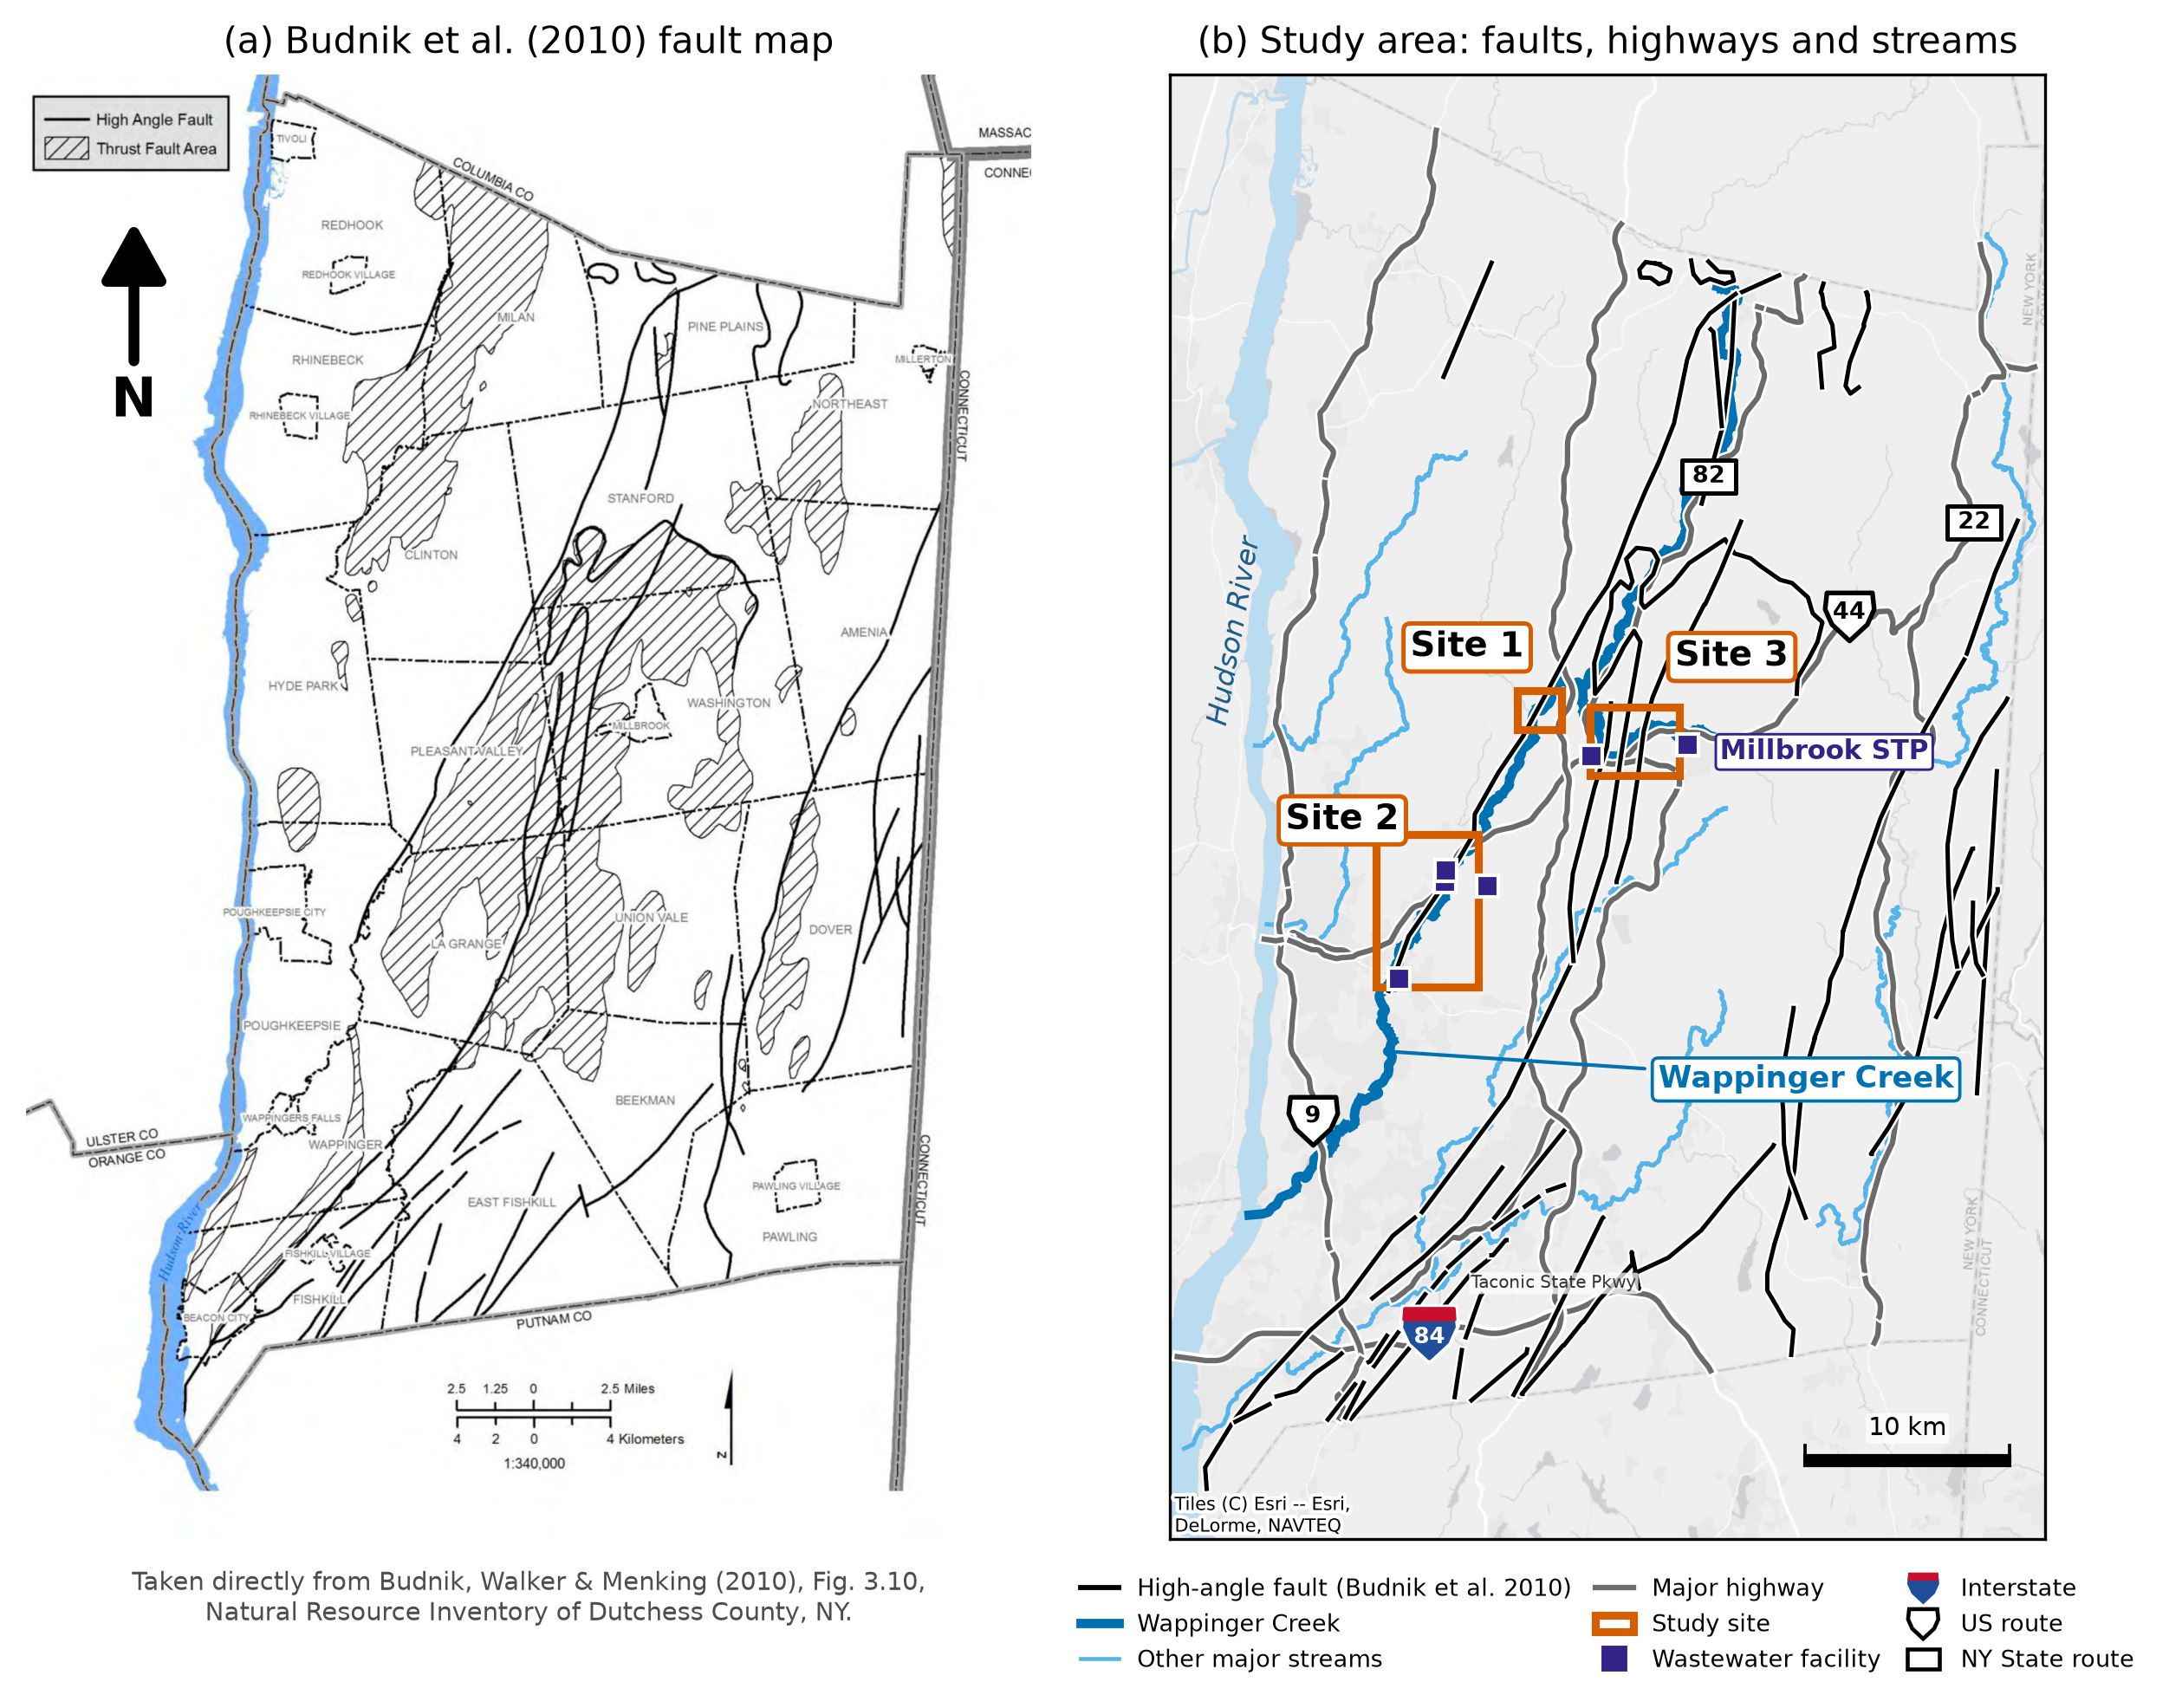
\includegraphics[width=\linewidth]{figures/rev_overview.png}
	\caption{Study area. The three study reaches (orange boxes) on Wappinger Creek, with high-angle faults digitized from \citet{budnik2010}, Fig.~3.10, wastewater facilities (squares) and major highways. STP is a sewage treatment plant. Sources: US Geological Survey National Hydrography Dataset; US Census Bureau TIGER/Line files; US Environmental Protection Agency Enforcement and Compliance History Online (ECHO) database; Esri.}
	\label{fig:overview}
\end{figure}

\subsection{In-situ sampling}\label{sec:sampling}

\linelabel{L:m-dates}Conductivity measurements were made on four days in autumn 2018: Site 1 on 28 September, Site 2 on 5 October, and Site 3 on 19 and 26 October. Site 3 was surveyed over two days, and it therefore comprises three surveys: one on 19 October, and two on 26 October, an upper survey that repeats Zones 3-1 and 3-2 and a lower survey that continues downstream from the end of the 19 October survey. Site 1 was surveyed at very high flow after rain and Site 2 at very high flow, whereas Site 3 was surveyed at baseflow on both days. We measured from upstream to downstream, traversing either on foot inside or around the creek or floating along the channel, and we sampled in the thalweg at each site to reduce variation due to incomplete lateral mixing. We used specific conductance as a proxy for salinity, and thus inferred changes in the salt input to the stream along its length from changes in specific conductance. We used a Thermo Scientific Orion 013010MD conductivity cell, calibrated following the standard protocols outlined by the manufacturer, with readings temperature-compensated to 25~$^{\circ}$C and reported as specific conductance (SC). \linelabel{L:m-accuracy}We did not record the meter model, but the Orion meters compatible with this cell specify an accuracy of $\pm$0.5\% of reading $\pm$1 digit, about $\pm$1.7~$\mu$S/cm at 310~$\mu$S/cm. A calibration offset shared by all readings on one day cancels when zones are compared within that day, while random reading error does not.

Mean spacing between points was about 85~m at Site 1, 416~m at Site 2 and 83--118~m on the Site 3 surveys, yielding 9, 18, and 46 measurement points at Sites 1, 2, and 3, respectively, with point positions recorded using a handheld GPS unit. Along-channel distance for each survey was computed by summing great-circle distances between consecutive GPS fixes in survey order, with the surveys that were walked upstream reversed so that distance increases downstream.

Within each site we delineated zones bounded at fault positions interpreted in the field or where the creek receives an active tributary, so that the reaches immediately upstream and downstream of a single geologic or hydrologic feature could be compared directly. To isolate the effect of faults, we restricted our fault-crossing contrasts to reaches where the creek intersects a mapped fault without a coincident tributary, because a tributary confluence introduces an independent salinity signal that would confound the comparison. At Site 1 a tributary enters where the channel meets the mapped fault, so we class its only contrast as a tributary contrast and do not count it among the fault contrasts. Because the fault traces are mapped at county scale, we treated each crossing as a reach-scale rather than a point-scale feature. We placed each fault boundary at an abrupt, roughly right-angle turn of the channel, which we took to be the creek turning to follow a fault; these field positions lie within a few hundred meters of, but not exactly at, the digitized trace crossings. \linelabel{L:site2-bend}At Site 2 the digitized county-scale trace runs along the creek for the whole surveyed reach, so it cannot resolve where the fault crosses the channel. The boundary between Zones 2-1 and 2-2, about 4~km along the survey, is therefore placed at the most abrupt bend on the reach, a roughly 90$^{\circ}$ turn of the channel. \linelabel{L:site2-bend-caveat}An abrupt bend is consistent with structural control of the channel, but it does not by itself show that groundwater flows along the fault there.

Zones are numbered so that they ascend downstream: for example, Zone 3-3 is downstream of Zone 3-2, which is downstream of Zone 3-1. This gives five upstream/downstream contrasts (Table~\ref{tab:ttest}): A (Zones 1-1/1-2, tributary), B (2-1/2-2, fault), C (3-1/3-2, tributary), D (3-2/3-3, first fault) and E (3-3/3-4, second fault). During the surveys we also marked the points that we believed lay just downstream of a fault, and we call these fault points (Figures~\ref{fig:site1}--\ref{fig:chloride} and Appendix A). \linelabel{L:faultpoints}They record our judgment on the day and not an observed fault position, and they do not enter the statistical tests; we use them only as a reference when reporting where a change in conductance or chloride lies. At Site 2, where the mapped fault zone runs along the creek, the fault points include three at the upstream end of Zone 2-1, where the mapped fault zone first meets the creek, as well as points in Zone 2-2. These upstream points do not define a second contrast: Site 2 has a single contrast, B, at the bend.

On 20 July 2020 we measured chloride along a 2.35~km transect of the East Branch at Site 3, from point Z (0~m) to point Z$'$ (2{,}351~m), passing the long-term monitoring site of \citet{kelly2019} at about 1{,}224~m (Figure~\ref{fig:chloride}). The aim was to see whether chloride rose near the mapped faults. We took 18 samples in the main channel and one in a side tributary. \linelabel{L:cl-sensor}Chloride was measured with a calibrated YSI Pro Series 1005 chloride ion-selective electrode (YSI 605105) on a YSI handheld meter. \linelabel{L:cl-accuracy}The manufacturer gives an accuracy of $\pm$15\% of reading or $\pm$5~mg/L, whichever is greater, which at our concentrations (about 14--50~mg/L) is $\pm$5 to $\pm$7.5~mg/L, so differences of a few mg/L between neighboring samples are within instrument error.

We sampled the transect in midsummer, when we expect streamflow to be dominated by baseflow and elevated chloride to come from groundwater more plausibly than from runoff, although we did not measure flow on that day. \linelabel{L:cl-single}Because it is a single transect from a different year than the conductivity survey, it cannot confirm the conductivity pattern, and we treat it as descriptive.

\subsection{Statistical analysis}
\label{sec:stats}

The zone contrasts and the change-point analysis described below address the first prediction, an abrupt rise at a fault. The second prediction can be examined only at Site 3, which was surveyed at baseflow, and the chloride transect bears on the third. \linelabel{L:m-welch}For each contrast we applied a two-sample Welch $t$-test (Equation~\ref{eq:ttest}) to evaluate the difference in mean specific conductance, in $\mu$S/cm, upstream and downstream of each feature. Unlike Student's pooled $t$-test, Welch's version does not assume equal variances and remains reliable with unequal sample sizes, as ours are, and is recommended as the default two-sample test \citep{ruxton2006}.

\begin{equation}
	t = \frac{\overline{x}_{2} - \overline{x}_{1}}
	         {\sqrt{\dfrac{s_{1}^{2}}{n_{1}} + \dfrac{s_{2}^{2}}{n_{2}}}}
	\label{eq:ttest}
\end{equation}

Here $\overline{x}_{1}$ and $\overline{x}_{2}$ are the mean specific conductance of the upstream and downstream zones, $s_{1}$ and $s_{2}$ their standard deviations, and $n_{1}$ and $n_{2}$ their sample sizes. \linelabel{L:m-withinday}Zones are compared only within a single survey day. Synoptic comparisons along a stream assume steady conditions, because concentrations that change between sampling runs are a source of uncertainty in a longitudinal profile \citep{runkel2013}. \linelabel{L:m-offset}This matters at Site 3, where conductance on the two survey days differed by about 28~$\mu$S/cm (Section~\ref{sec:contrasts}), which is larger than any of the contrasts we test. We chose not to pool the two days or to subtract the offset, because the reach surveyed on both days shows that the offset is not constant along the channel. Thus, Contrast D is tested on 19 October and Contrast E on 26 October. Zone 3-3 was surveyed partly on each day, however, so the simplest analysis would pool the two days into one Site 3 data set. To show what that choice does, we also ran the Contrast E test on the pooled data, and we report it separately in Section~\ref{sec:contrasts}. We evaluated significance with two-tailed tests at $\alpha = 0.05$. Because our zone samples are relatively small and not guaranteed to be normally distributed, we accompanied every Welch test with a distribution-free Mann--Whitney $U$ test and regard a contrast as robust only where the two approaches agree, which guards against over-interpreting the smaller contrasts.

\linelabel{L:m-autocorr}Applying a $t$-test to measurements collected sequentially along a channel warrants caution, because closely spaced samples are not strictly independent and nominal $p$-values are therefore likely too small. For each contrast we estimated the lag-1 autocorrelation $\rho$ of the residuals from the two zone means, pooled in along-channel order. Negative values were set to zero and $\rho$ was capped at 0.9. We then computed an effective sample size for each zone, $n_{\mathrm{eff}} = n(1-\rho)/(1+\rho)$, floored at 2 and not exceeding $n$, and repeated the Welch test with $n_{\mathrm{eff}}$ in place of $n$ (degrees of freedom by the Welch--Satterthwaite approximation). \linelabel{L:m-autocorr-check}With zones of three to eleven points, $\rho$ is poorly determined, so we treat the adjusted $p$-values as a sensitivity check rather than a correction.

\linelabel{L:m-changepoint}Zone means cannot show whether a change in conductance is abrupt or gradual, so we also looked for change points along each transect. For each single-day transect separately (Site 1, Site 2, the 19 October survey at Site 3, and the upper and lower 26 October surveys at Site 3), we fitted continuous piecewise-linear regressions of specific conductance on along-channel distance with zero, one, or two breakpoints, requiring at least three points in each segment, and chose the number of breakpoints by the Bayesian information criterion (BIC). Uncertainty in each breakpoint was assessed with a residual bootstrap (500 replicates). As an independent check we applied a penalized change-in-mean analysis (the pruned exact linear time, or PELT, algorithm in the \texttt{ruptures} package). The same procedure was applied to the chloride transect.

Finally, because roads are a possible alternative source of the conductance differences, we computed the distance from each survey point to the nearest major road, defined as primary or secondary roads (US Census Bureau TIGER/Line 2024 road files, feature classes S1100 and S1200; the Taconic State Parkway is coded as a local road, S1400, and is therefore excluded). We report these distances descriptively by zone and do not test them.

\section{Results}

\subsection{Within-day zone contrasts}\label{sec:contrasts}

In the following, we first report the zone contrasts survey by survey, then show what pooling the two Site 3 days does to them, and lastly describe the reach that was surveyed on both days. \linelabel{L:table-intro}Table~\ref{tab:ttest} gives each contrast with zone means $\pm$ SD and the number of points $n$; Table~\ref{tab:support} gives the autocorrelation-adjusted $p$-values and the median distance from each zone's points to the nearest major road; Appendix~A lists every measurement. \linelabel{L:sd-range}Within a single day the zone standard deviations are 0.1--2.6~$\mu$S/cm.

% Tables 1 and 2 follow the paragraph that introduces them.
\begin{table}[htbp]
	\caption{Within-day zone contrasts in specific conductance ($\mu$S/cm). $\Delta$ is downstream minus upstream, with its Welch 95\% CI; $U$ and $p_{\mathrm{MW}}$ are from the Mann--Whitney test. $^\dagger$ marks a zone with fewer than five points.}
	\centering
	\scriptsize
	\setlength{\tabcolsep}{3pt}
	\resizebox{\linewidth}{!}{% Auto-generated by src/within_day.py -- do not edit by hand.
% Within-single-day contrasts. Delta = downstream - upstream (uS/cm). n<=3 in a zone: interpret with great caution.
\begin{tabular}{llllrrrrrrrr}
\toprule
Contr. & Boundary & Date & Zones & $n_1,n_2$ & Up (mean$\pm$SD) & Down (mean$\pm$SD) & $\Delta$ [95\% CI] & Welch $t$ (df) & $p$ & $U$ & $p_{\mathrm{MW}}$ \\
\midrule
A & tributary & 28 Sep & 1-1$\rightarrow$1-2 & 4,5$^{\dagger}$ & 259.9$\pm$0.7 & 259.4$\pm$0.1 & -0.5 [-1.5, +0.6] & -1.35 (3.2) & 0.264 & 5 & 0.266 \\
B & fault & 5 Oct & 2-1$\rightarrow$2-2 & 10,8 & 308.8$\pm$1.1 & 313.1$\pm$1.9 & +4.3 [+2.6, +6.0] & 5.63 (10.8) & $<$0.001 & 79 & $<$0.001 \\
C & tributary & 19 Oct & 3-1$\rightarrow$3-2 & 6,3$^{\dagger}$ & 340.1$\pm$0.4 & 336.3$\pm$2.2 & -3.8 [-9.2, +1.5] & -2.97 (2.1) & 0.093 & 0 & 0.028 \\
C & tributary & 26 Oct & 3-1$\rightarrow$3-2 & 11,3$^{\dagger}$ & 370.5$\pm$2.6 & 364.9$\pm$1.1 & -5.6 [-7.9, -3.3] & -5.48 (8.8) & $<$0.001 & 0 & 0.012 \\
D & fault & 19 Oct & 3-2$\rightarrow$3-3 & 3,11$^{\dagger}$ & 336.3$\pm$2.2 & 333.4$\pm$1.9 & -2.8 [-7.4, +1.7] & -2.02 (2.9) & 0.140 & 6 & 0.119 \\
E & fault & 26 Oct & 3-3$\rightarrow$3-4 & 6,6 & 358.8$\pm$1.8 & 360.4$\pm$0.8 & +1.6 [-0.3, +3.4] & 1.96 (7.0) & 0.090 & 30 & 0.076 \\
\bottomrule
\end{tabular}
% $^{\dagger}$ one zone has fewer than 5 points (add to the caption).
}
	\label{tab:ttest}
\end{table}

\begin{table}[htbp]
	\caption{Autocorrelation-adjusted tests and road distances for Table~\ref{tab:ttest}. $\hat\rho_1$ is the lag-1 autocorrelation and $n_{\mathrm{eff}} = n(1-\rho)/(1+\rho)$ the effective sample size; adjusted $p$-values are a sensitivity check. Road distances are zone medians to the nearest primary or secondary road and were not tested.}
	\centering
	\small
	% Auto-generated by src/within_day.py -- do not edit by hand.
\begin{tabular}{lllrrrrrrr}
\toprule
Contr. & Date & Zones & $\hat\rho_1$ & $n_{\mathrm{eff},1}$ & $n_{\mathrm{eff},2}$ & $p$ (Welch) & $p$ ($n_{\mathrm{eff}}$) & \multicolumn{2}{c}{Median road dist. (m)} \\
\cmidrule(lr){9-10}
 & & & & & & & & up & down \\
\midrule
A & 28 Sep & 1-1$\rightarrow$1-2 & -0.27 & 4.0 & 5.0 & 0.264 & 0.264 & 927 & 751 \\
B & 5 Oct & 2-1$\rightarrow$2-2 & 0.37 & 4.6 & 3.7 & $<$0.001 & 0.017 & 335 & 726 \\
C & 19 Oct & 3-1$\rightarrow$3-2 & -0.35 & 6.0 & 3.0 & 0.093 & 0.093 & 304 & 425 \\
C & 26 Oct & 3-1$\rightarrow$3-2 & 0.54 & 3.2 & 2.0 & $<$0.001 & 0.041 & 245 & 414 \\
D & 19 Oct & 3-2$\rightarrow$3-3 & 0.35 & 2.0 & 5.3 & 0.140 & 0.279 & 425 & 409 \\
E & 26 Oct & 3-3$\rightarrow$3-4 & 0.30 & 3.2 & 3.2 & 0.090 & 0.243 & 312 & 368 \\
\bottomrule
\end{tabular}

	\label{tab:support}
\end{table}

\textbf{Site 1, Contrast A (28 September).} At Site 1 the tributary contrast showed no detectable change. Specific conductance fell from 259.9 $\pm$ 0.7~$\mu$S/cm in Zone 1-1 ($n = 4$) to 259.4 $\pm$ 0.1~$\mu$S/cm in Zone 1-2 ($n = 5$), a change of $-0.5$~$\mu$S/cm that is not significant (Figure~\ref{fig:site1}; Table~\ref{tab:ttest}). A tributary enters at the same place where the channel turns along the mapped fault trace, and Site 1 was at very high flow after rain; conductance there was 50--100~$\mu$S/cm lower than at the other sites, consistent with dilution by runoff, so this contrast cannot isolate a fault effect and, with four and five points, has little power.

\begin{figure}[htbp]
	\centering
	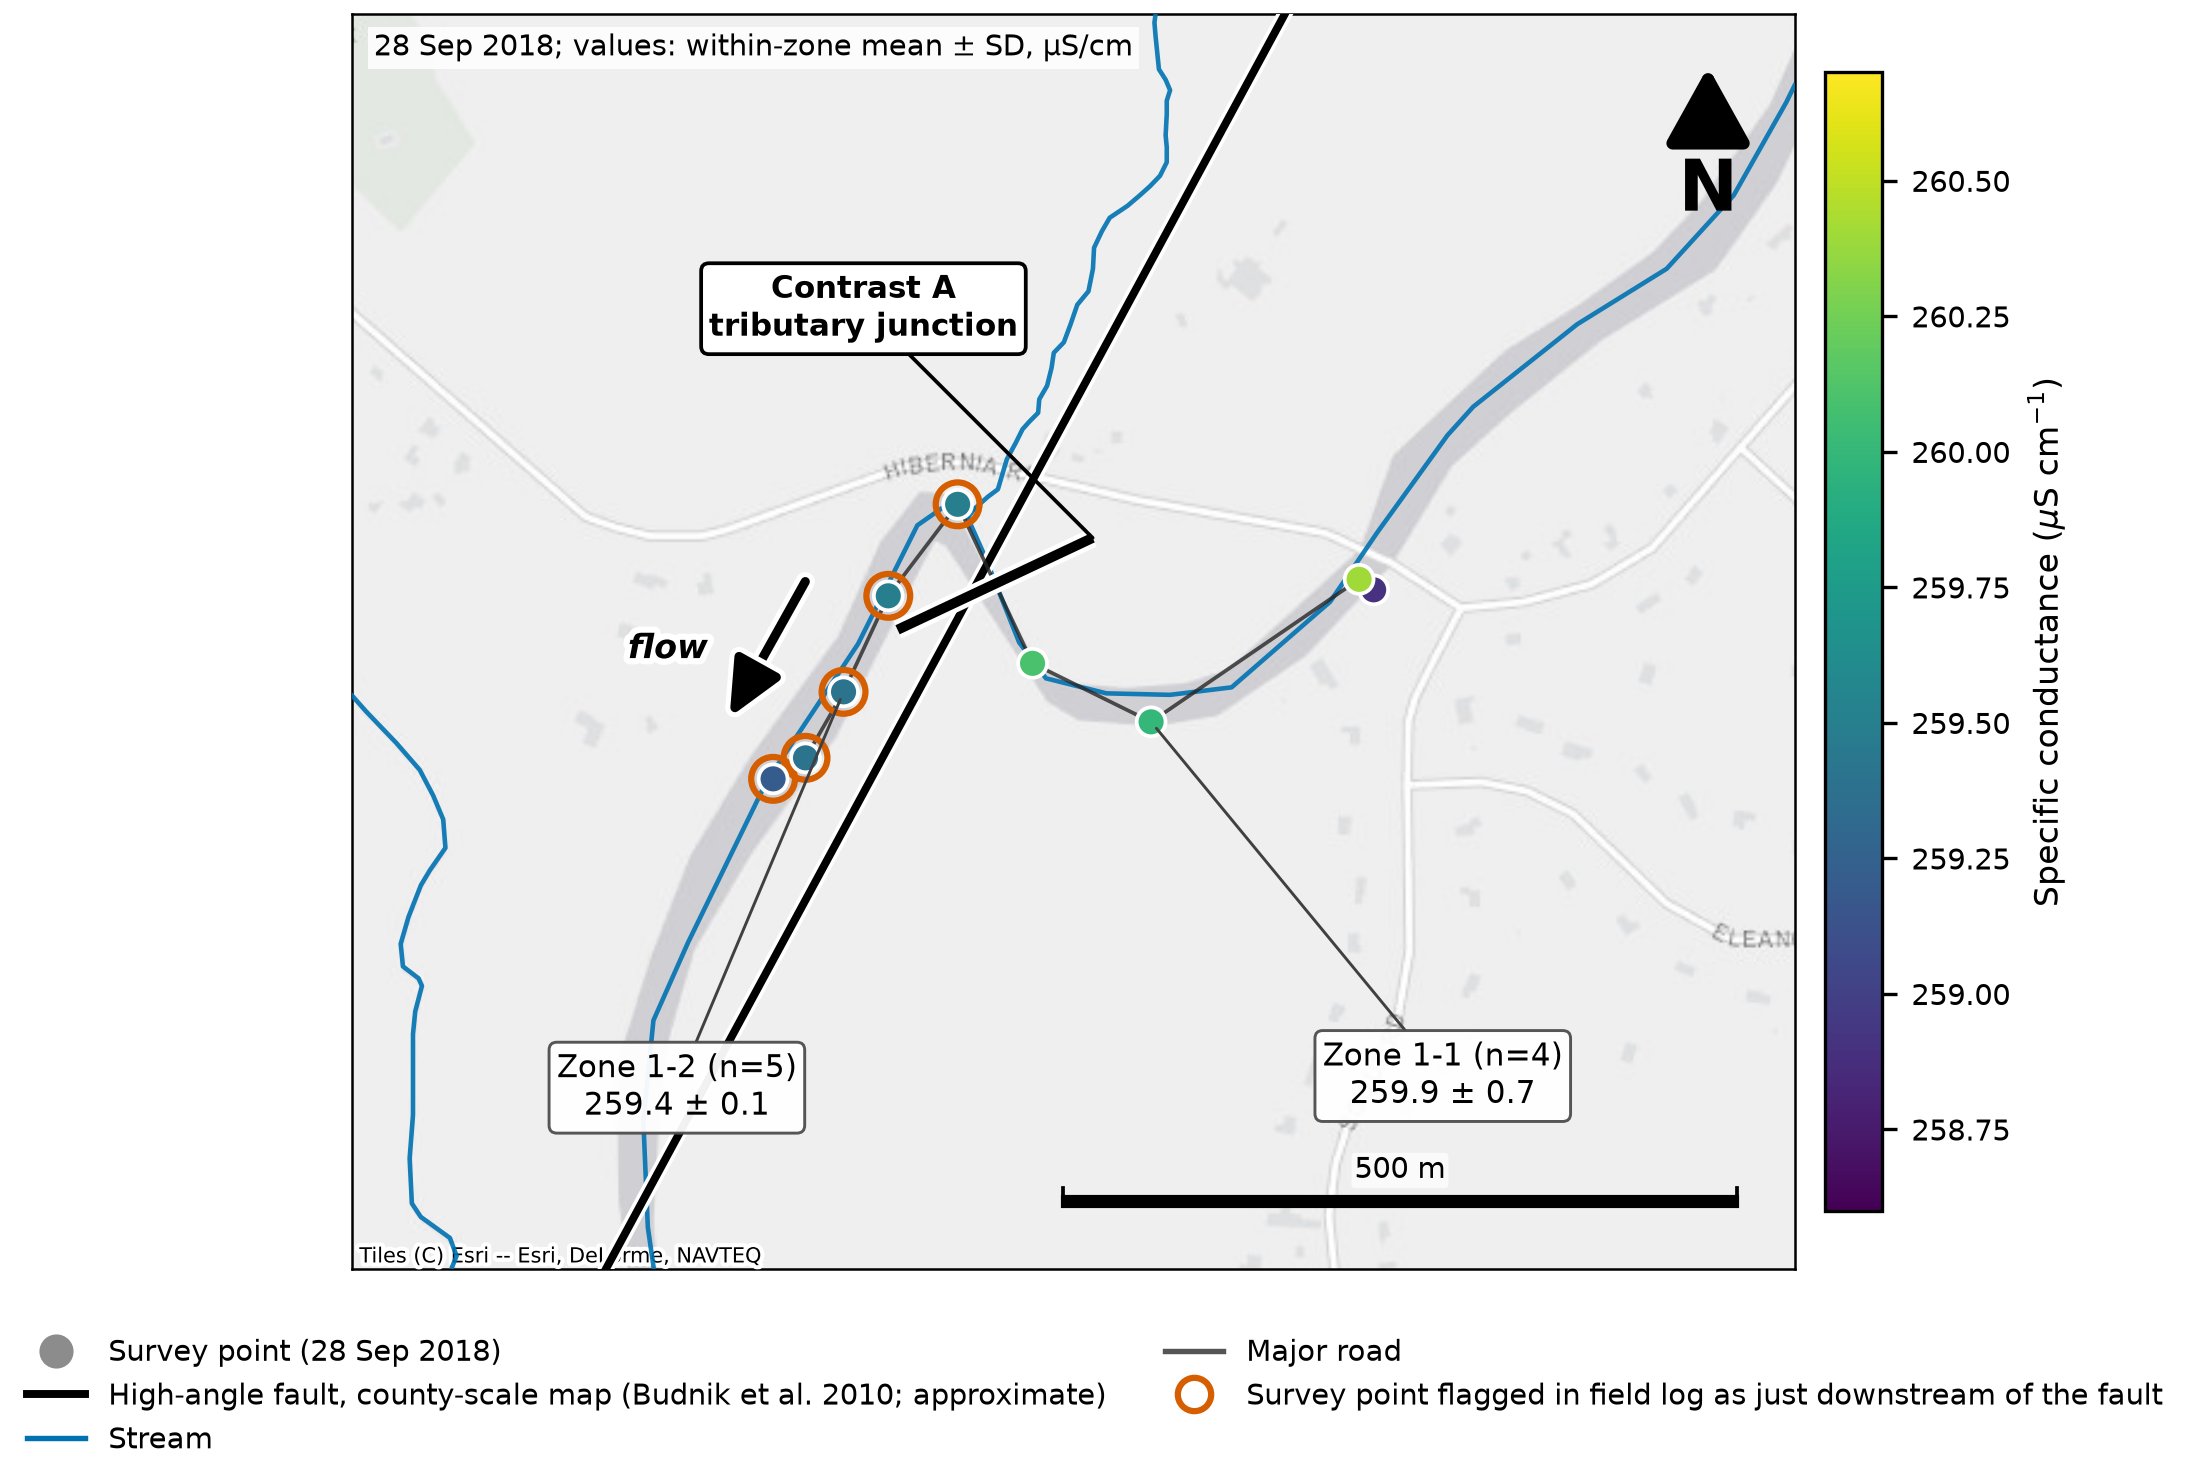
\includegraphics[width=0.7\linewidth]{figures/rev_site1.png}
	\caption{Site 1 (28 September 2018) and Contrast A. Points are colored by specific conductance; orange rings mark fault points. Zone labels give $n$ and mean $\pm$ SD ($\mu$S/cm). Faults from \citet{budnik2010}.}
	\label{fig:site1}
\end{figure}

\textbf{Site 2, Contrast B (5 October).} Site 2 gave the only significant increase at a fault. Zone 2-1 averaged 308.8 $\pm$ 1.1~$\mu$S/cm ($n = 10$) and Zone 2-2 averaged 313.1 $\pm$ 1.9~$\mu$S/cm ($n = 8$), an increase of $+4.3$~$\mu$S/cm (95\% CI $+2.6$ to $+6.0$; Welch $p < 0.001$; Mann--Whitney $p < 0.001$; Figure~\ref{fig:site2}). \linelabel{L:contrastB-adj}Allowing for autocorrelation along the channel ($n_{\mathrm{eff}} = 4.6$ and 3.7), the adjusted $p$ is 0.017 (Table~\ref{tab:support}). The difference is larger than the within-zone standard deviations and about 2.5 times the instrument's stated accuracy at this conductance. The Zone 2-1/2-2 boundary, about 4.0~km along the survey, is the channel bend described in Section~\ref{sec:sampling}. \linelabel{L:site2-trace}The digitized county-scale trace runs along the creek throughout and crosses the survey line at about 1.0 and 5.8~km, but those intersections are not reliable fault positions, so we did not use them. \linelabel{L:site2-flow}Flow was very high for the duration of the Site 2 survey, and we canoed part of it, so this survey may not represent baseflow.

\begin{figure}[htbp]
	\centering
	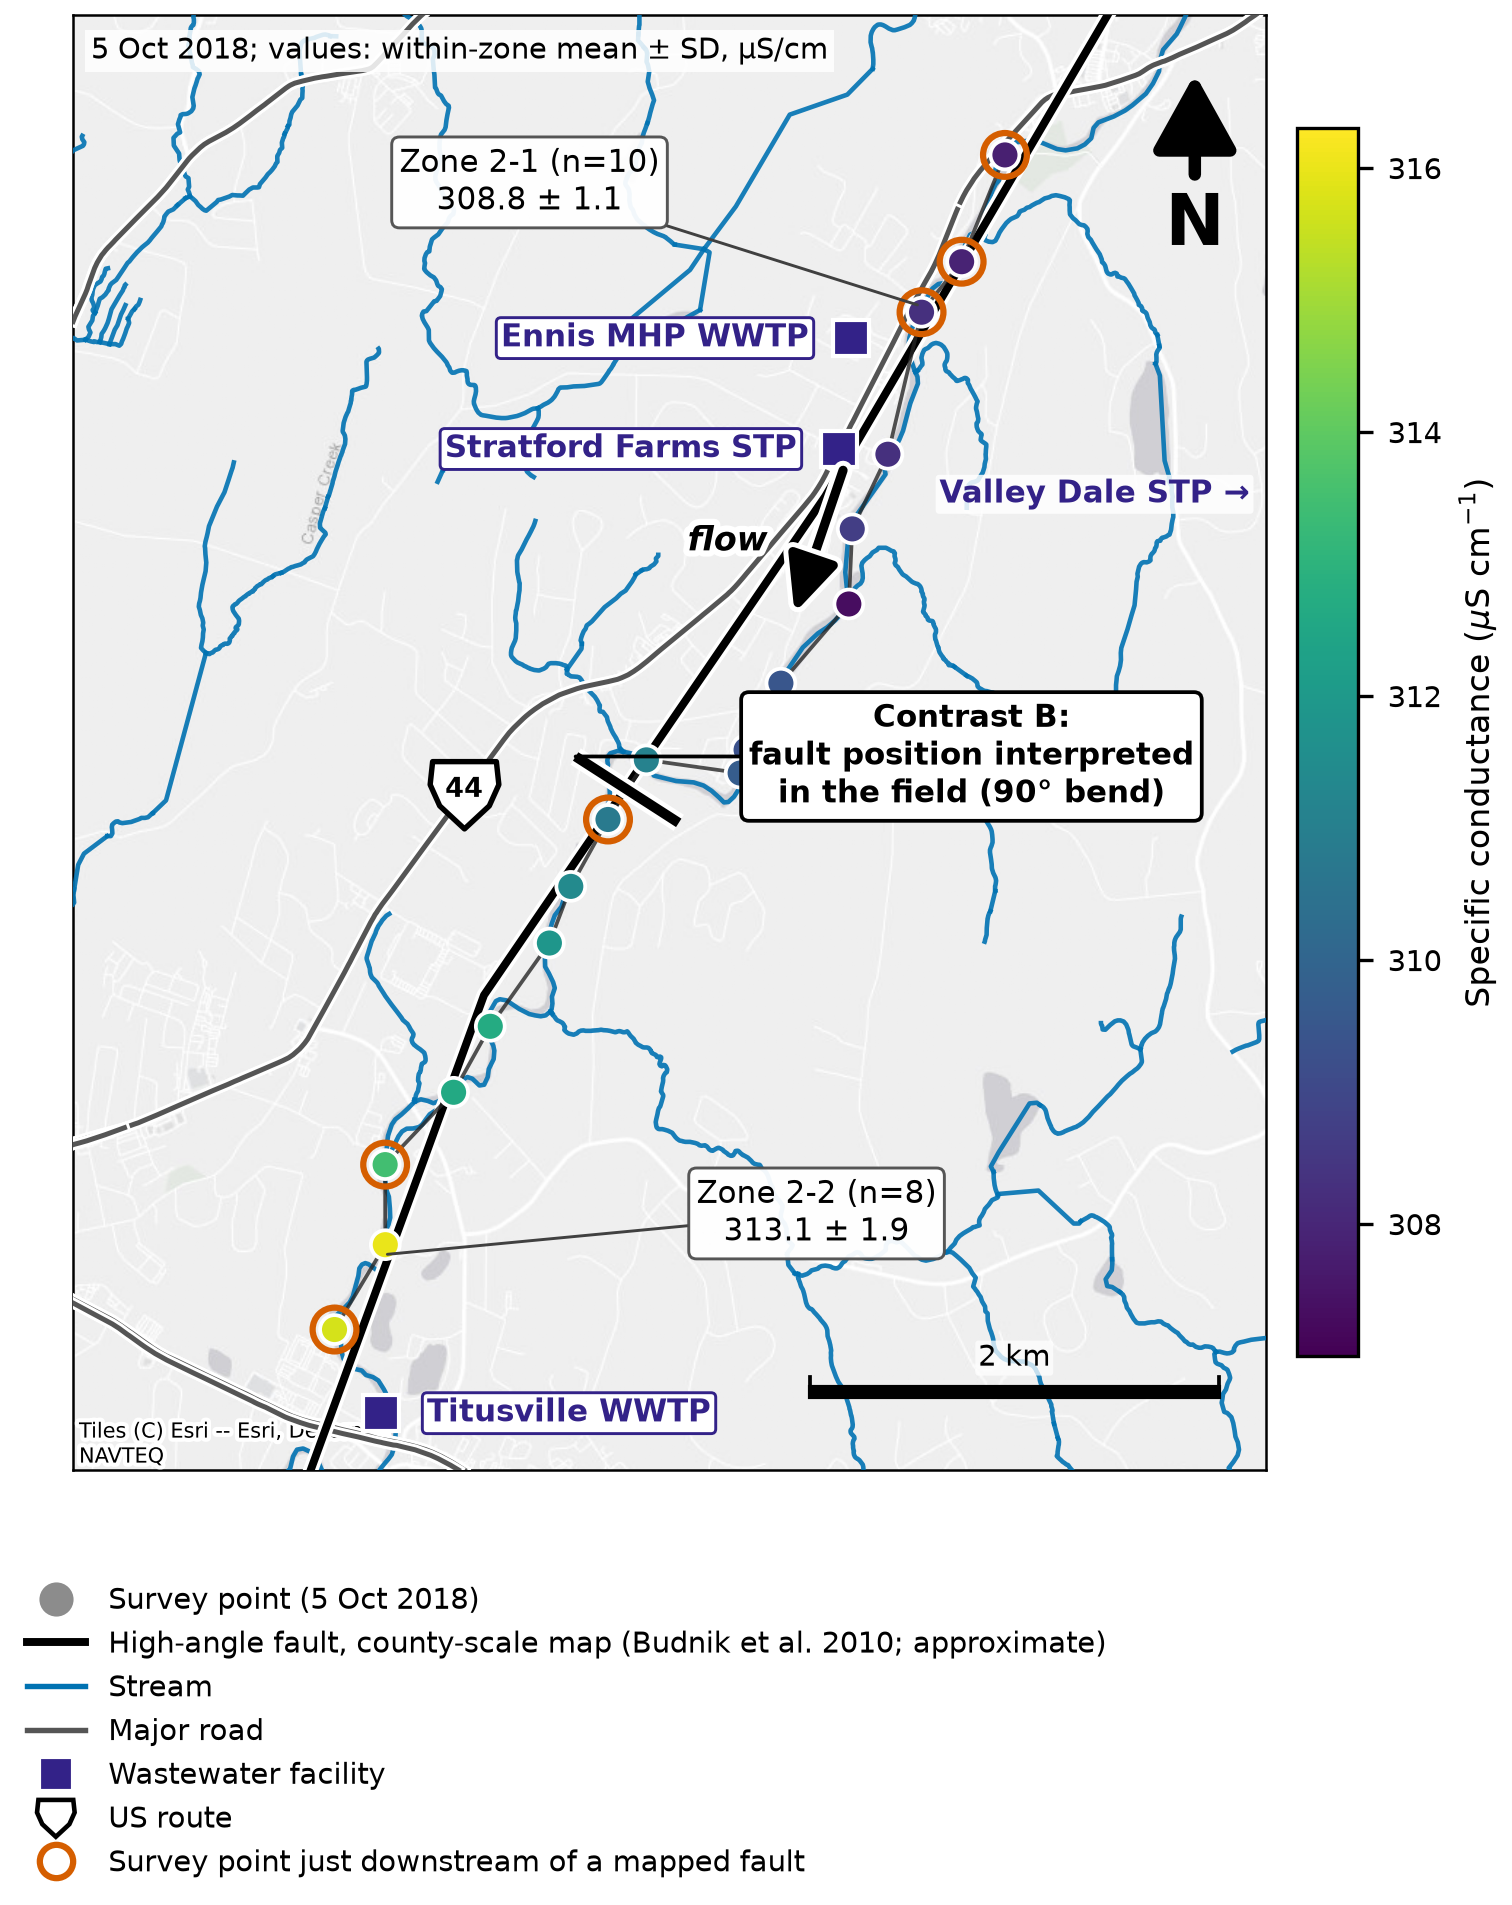
\includegraphics[width=0.78\linewidth]{figures/rev_site2.png}
	\caption{Site 2 (5 October 2018) and Contrast B. Symbols as in Figure~\ref{fig:site1}. The zone boundary is the fault position interpreted in the field at an abrupt 90$^{\circ}$ bend. The fault points at the upstream end of Zone 2-1 lie where the mapped fault zone first meets the creek and do not define a second contrast. Squares are wastewater facilities (STP, sewage treatment plant; WWTP, wastewater treatment plant; MHP, mobile home park).}
	\label{fig:site2}
\end{figure}

\textbf{Site 3, Contrasts C, D and E (19 and 26 October).} At Site 3 (Figure~\ref{fig:site3}), conductance fell at the tributary junction on both days, while neither fault contrast showed a significant increase. Contrast C, the tributary junction, is a decrease on both days: $-3.8$~$\mu$S/cm on 19 October (340.1 $\pm$ 0.4, $n = 6$, to 336.3 $\pm$ 2.2, $n = 3$; Welch $p = 0.093$; Mann--Whitney $p = 0.028$) and $-5.6$~$\mu$S/cm on 26 October (370.5 $\pm$ 2.6, $n = 11$, to 364.9 $\pm$ 1.1, $n = 3$; Welch $p < 0.001$; Mann--Whitney $p = 0.012$; adjusted $p = 0.041$). On 19 October the two tests disagree, and hence this contrast does not meet the robustness criterion of Section~\ref{sec:stats}. We believe the disagreement says more about the sample than about the stream, because with groups of only six and three points the Mann--Whitney test cannot return an exact $p$ below about 0.024, and the downstream zone has only three points on either day, so both tests have little power. Contrast D, the first fault, can be tested only on 19 October, because on 26 October Zones 3-2 and 3-3 lie on different transects 1.1~km apart. \linelabel{L:contrastD}It is a decrease of $-2.8$~$\mu$S/cm (336.3 $\pm$ 2.2, $n = 3$, to 333.4 $\pm$ 1.9, $n = 11$; 95\% CI $-7.4$ to $+1.7$; $p = 0.140$). Contrast E, the second fault, can be tested only on 26 October. Conductance rose from 358.8 $\pm$ 1.8~$\mu$S/cm ($n = 6$) in Zone 3-3 to 360.4 $\pm$ 0.8~$\mu$S/cm ($n = 6$) in Zone 3-4, \linelabel{L:contrastE}an increase of $+1.6$~$\mu$S/cm (95\% CI $-0.3$ to $+3.4$; Welch $p = 0.090$; Mann--Whitney $p = 0.076$; adjusted $p = 0.243$), which is not significant and within the instrument's stated accuracy ($\pm$1.9~$\mu$S/cm at 360~$\mu$S/cm). The tributary contrast (C) is thus in the direction mixing predicts, a decrease where the tributary, which measured nearly 150~$\mu$S/cm lower than Zones 3-1 and 3-2, enters, while neither Site 3 fault contrast shows a significant increase.

\begin{figure}[htbp]
	\centering
	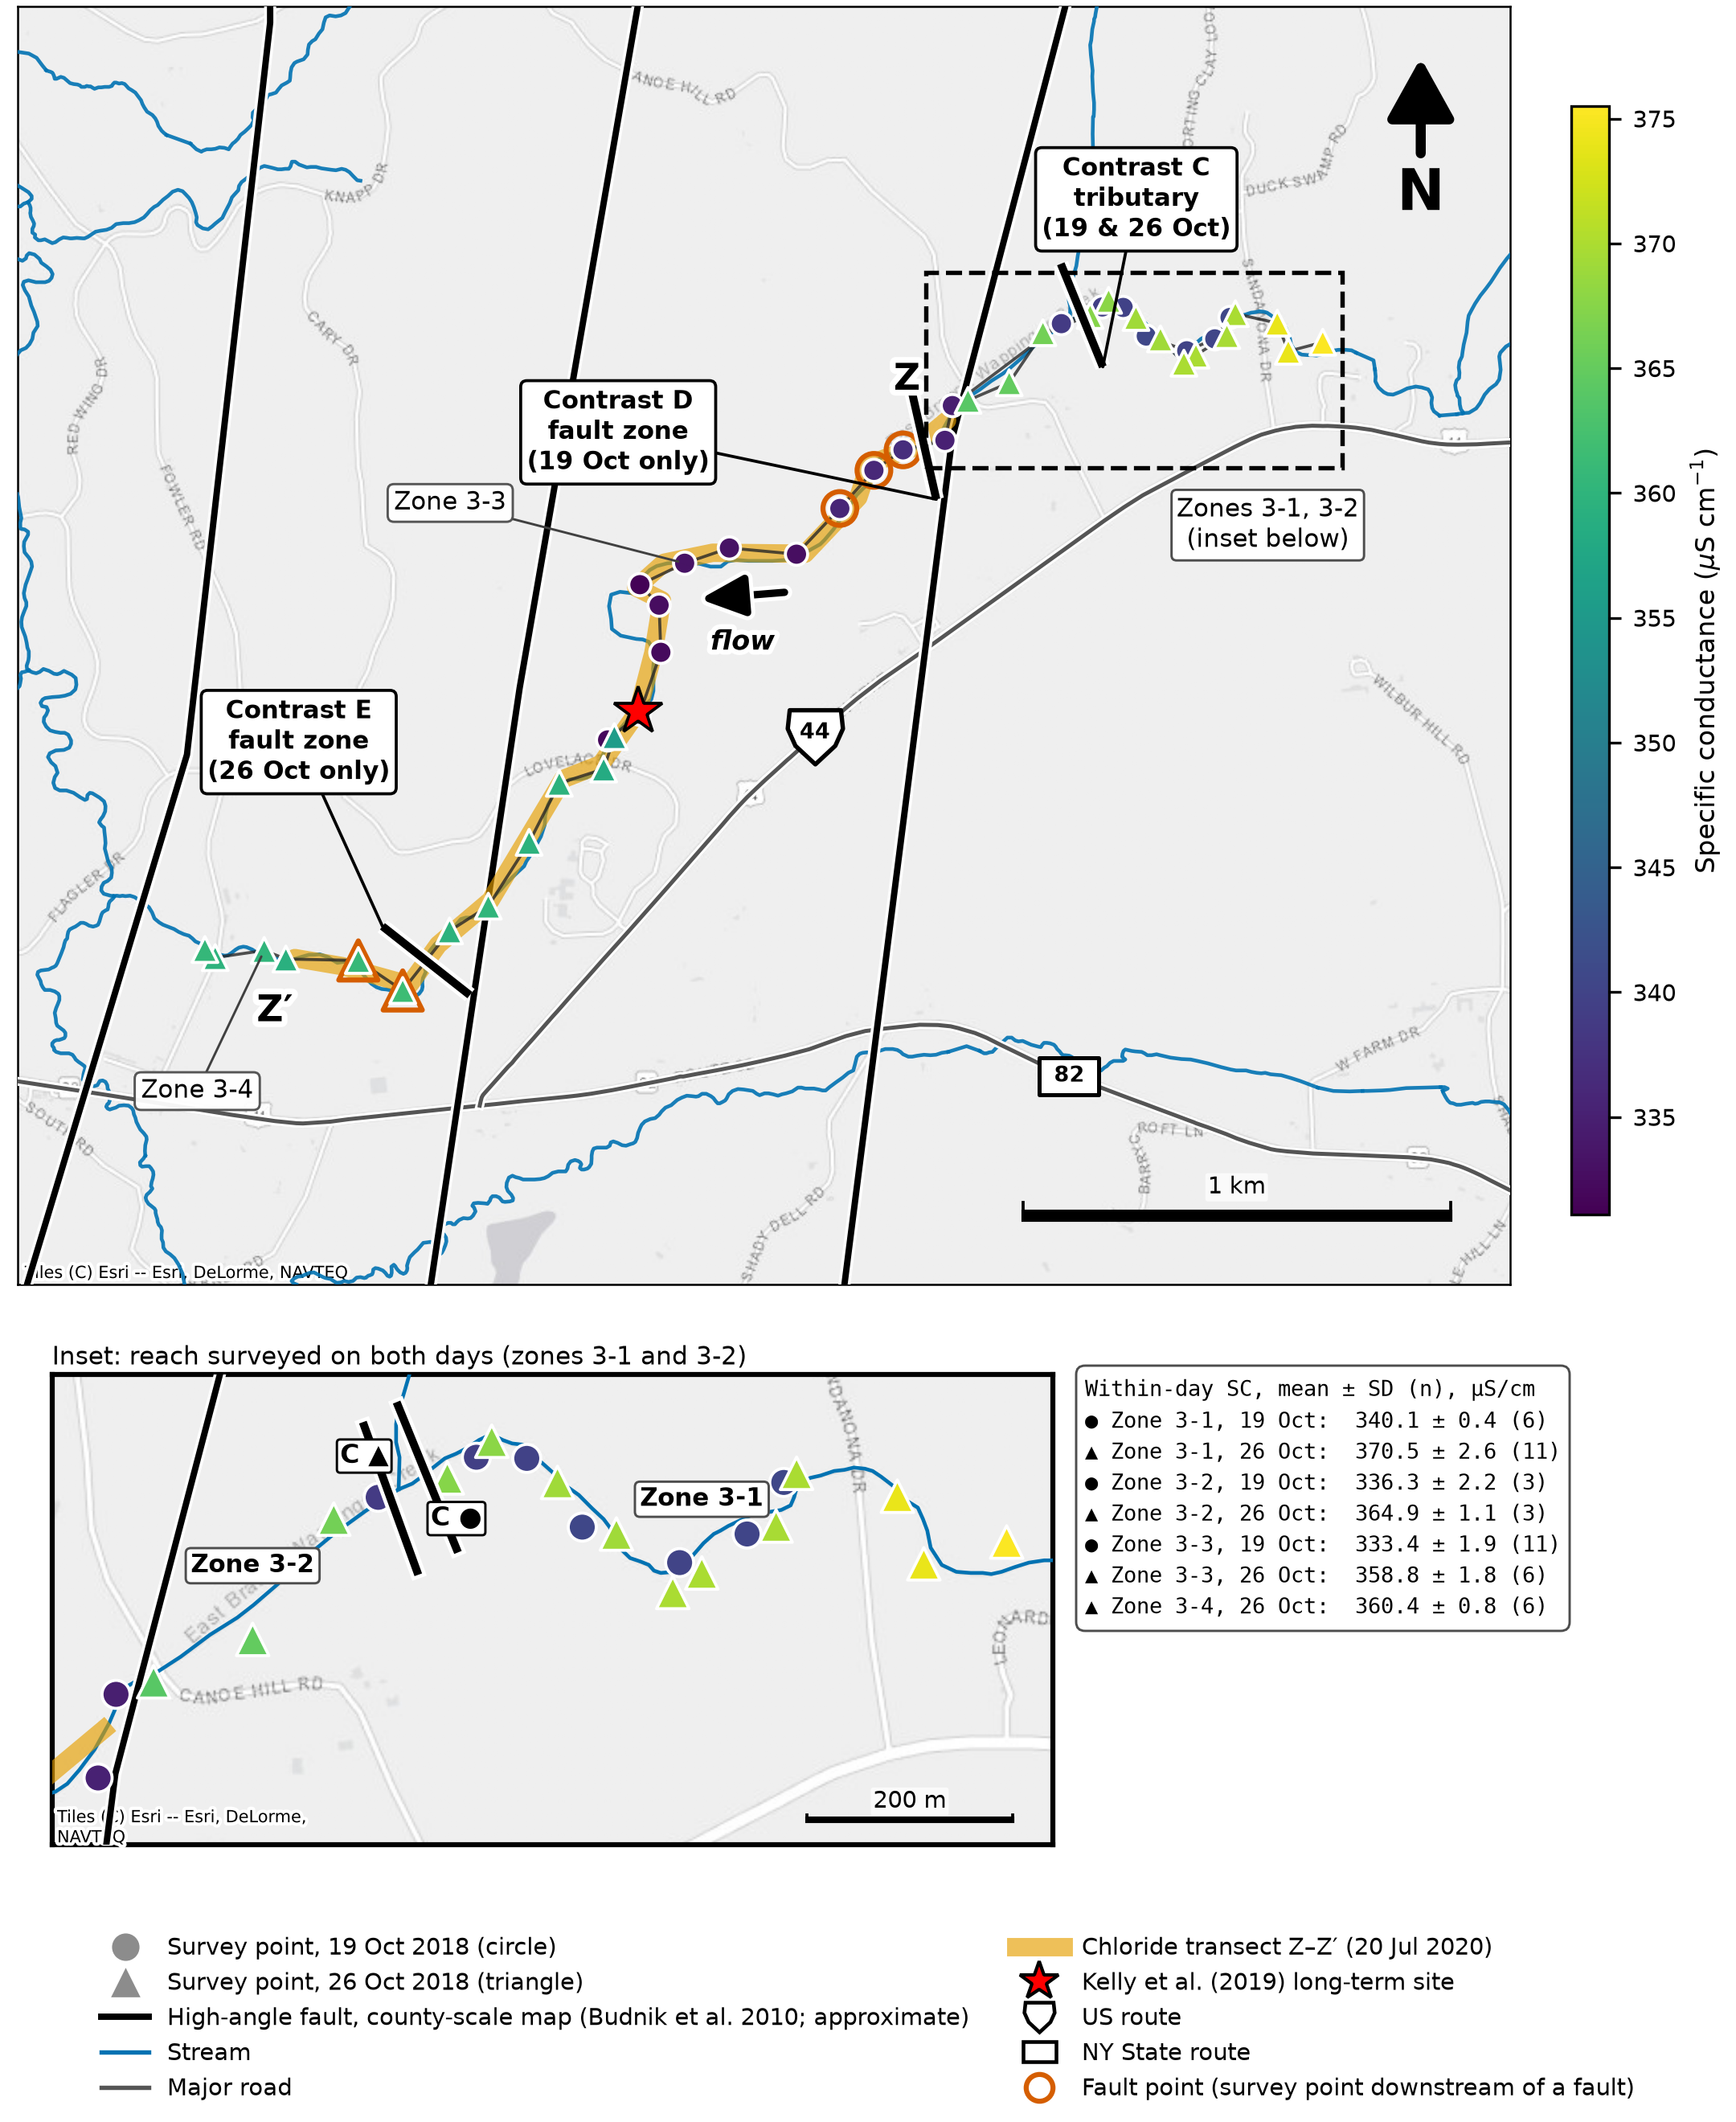
\includegraphics[width=0.85\linewidth]{figures/rev_site3.png}
	\caption{Site 3 and Contrasts C, D and E. Circles are 19 October and triangles 26 October 2018 points; the two days differ by about 28~$\mu$S/cm, so zones are compared within a day only. Orange rings mark fault points. The inset enlarges the reach surveyed on both days; the Contrast C boundary is drawn separately for each day because the survey points nearest the junction differ between days. The yellow band is the 2020 chloride transect (Z--Z$'$) and the red star the monitoring site of \citet{kelly2019}.}
	\label{fig:site3}
\end{figure}

\textbf{Pooling days.} The within-day rule matters most at Contrast E. \linelabel{L:pooling}When we pooled the two survey days, as a first analysis of the Site 3 data naturally would, Contrast E appeared as a rise of $+18.0$~$\mu$S/cm ($p < 0.001$), larger than any other step in the survey. However, this value is an artifact of the pooling: Zone 3-3 then combines 11 points from 19 October (333.4~$\mu$S/cm) with 6 from 26 October (358.8~$\mu$S/cm), giving a pooled mean of 342.4~$\mu$S/cm, while Zone 3-4 consists only of 26 October points. In other words, the ``step'' is the difference between days and not a change along the channel; \linelabel{L:pooling-sd}the same pooling inflates the zone standard deviations to 12.6--15.8~$\mu$S/cm, against 0.4--2.6~$\mu$S/cm within a day at Site 3.

\textbf{Day offset and the repeated reach.} \linelabel{L:offset-pairs}Eleven 19 October points have a 26 October point within 120~m, and the pairs differ by 23.5--29.7~$\mu$S/cm (mean 27.8, SD 2.2); \linelabel{L:offset-seam}two points 18~m apart at the seam between the surveys read 332.0 and 355.5~$\mu$S/cm. This seam falls inside Zone 3-3, which is why Figure~\ref{fig:site3} shows an abrupt change of color partway along that zone. Hence, the offset is not constant, and its range of about 6~$\mu$S/cm exceeds Contrasts B and E, which is why we neither pooled days nor corrected for it. We do not know what caused the offset: Site 3 was at baseflow on both days, and we have no discharge or other measurements with which to explain it. \linelabel{L:offset-repeat}Zones 3-1 and 3-2 were surveyed on both days (Figure~\ref{fig:site3}, inset): Zone 3-1 averaged 340.1 $\pm$ 0.4~$\mu$S/cm ($n = 6$) on 19 October and 370.5 $\pm$ 2.6 ($n = 11$) on 26 October, and Zone 3-2 averaged 336.3 $\pm$ 2.2 ($n = 3$) and 364.9 $\pm$ 1.1 ($n = 3$), so within each day the zones are internally consistent, while the zone means differ between days by about 29--30~$\mu$S/cm, close to the offset between the paired points.

\subsection{Change-point analysis of specific conductance}

\linelabel{L:cp-none}Segmented regression and a change-in-mean check on each single-day transect (Figure~\ref{fig:changepoint}) find no specific-conductance breakpoint at a fault contrast boundary or at a point where the digitized trace crosses the transect. \linelabel{L:cp-site2}At Site 2 one breakpoint is selected at 2{,}355~m (bootstrap interval 1{,}327--3{,}384~m), after which conductance rises steadily downstream; the fitted slope increases from 0.1 to 1.6~$\mu$S/cm per km. This breakpoint lies about 1.6~km upstream of the Contrast B boundary at 3{,}993~m, the field-interpreted fault position at the channel bend (between 0.6 and 2.7~km upstream, given the bootstrap interval); the change-in-mean analysis places three small shifts ($+1.5$, $+2.3$ and $+3.3$~$\mu$S/cm) between 2.6 and 5.9~km. \linelabel{L:cp-contrastB}Contrast B is therefore better described as part of a gradual downstream ramp than as an abrupt step at the interpreted fault position.

At the other sites, the analysis gave even less indication of a step. At Site 1 and on the 19 October Site 3 transect no breakpoint is selected (for 19 October a one-breakpoint model ties with none, $\Delta$BIC = 0.03). \linelabel{L:cp-19oct}Instead, on 19 October conductance fell downstream along most of the transect, from 340.5~$\mu$S/cm at its upstream end to 332.0~$\mu$S/cm at its downstream end, through both the tributary junction and the Contrast D boundary, which is the opposite of what a salt-laden fault input would produce. On the upper 26 October Site 3 transect two breakpoints (300 and 459~m) are only marginally preferred ($\Delta$BIC = 0.3) and lie 314--473~m upstream of the tributary junction and away from any trace. \linelabel{L:cp-trib}The tributary junction thus fares only slightly better than the faults by this test: the change-in-mean analysis places a shift of $-3.2$~$\mu$S/cm at the junction on 26 October, but on 19 October neither method places a change there, and conductance was already falling upstream of the junction on both days. On the lower 26 October transect (Contrast E) one breakpoint is selected at 194~m, where conductance rises from 355.5 to 359.7~$\mu$S/cm over the first 190~m and then stays near 360~$\mu$S/cm. This breakpoint is not at the fault by any measure we have. \linelabel{L:cp-E-min}This breakpoint sits at the three-point minimum segment the method allows, 330~m upstream of where the channel crosses the digitized trace (at 523~m), 123~m in straight-line distance from the nearest trace, and 522~m upstream of the Contrast E boundary.

\begin{figure}[htbp]
	\centering
	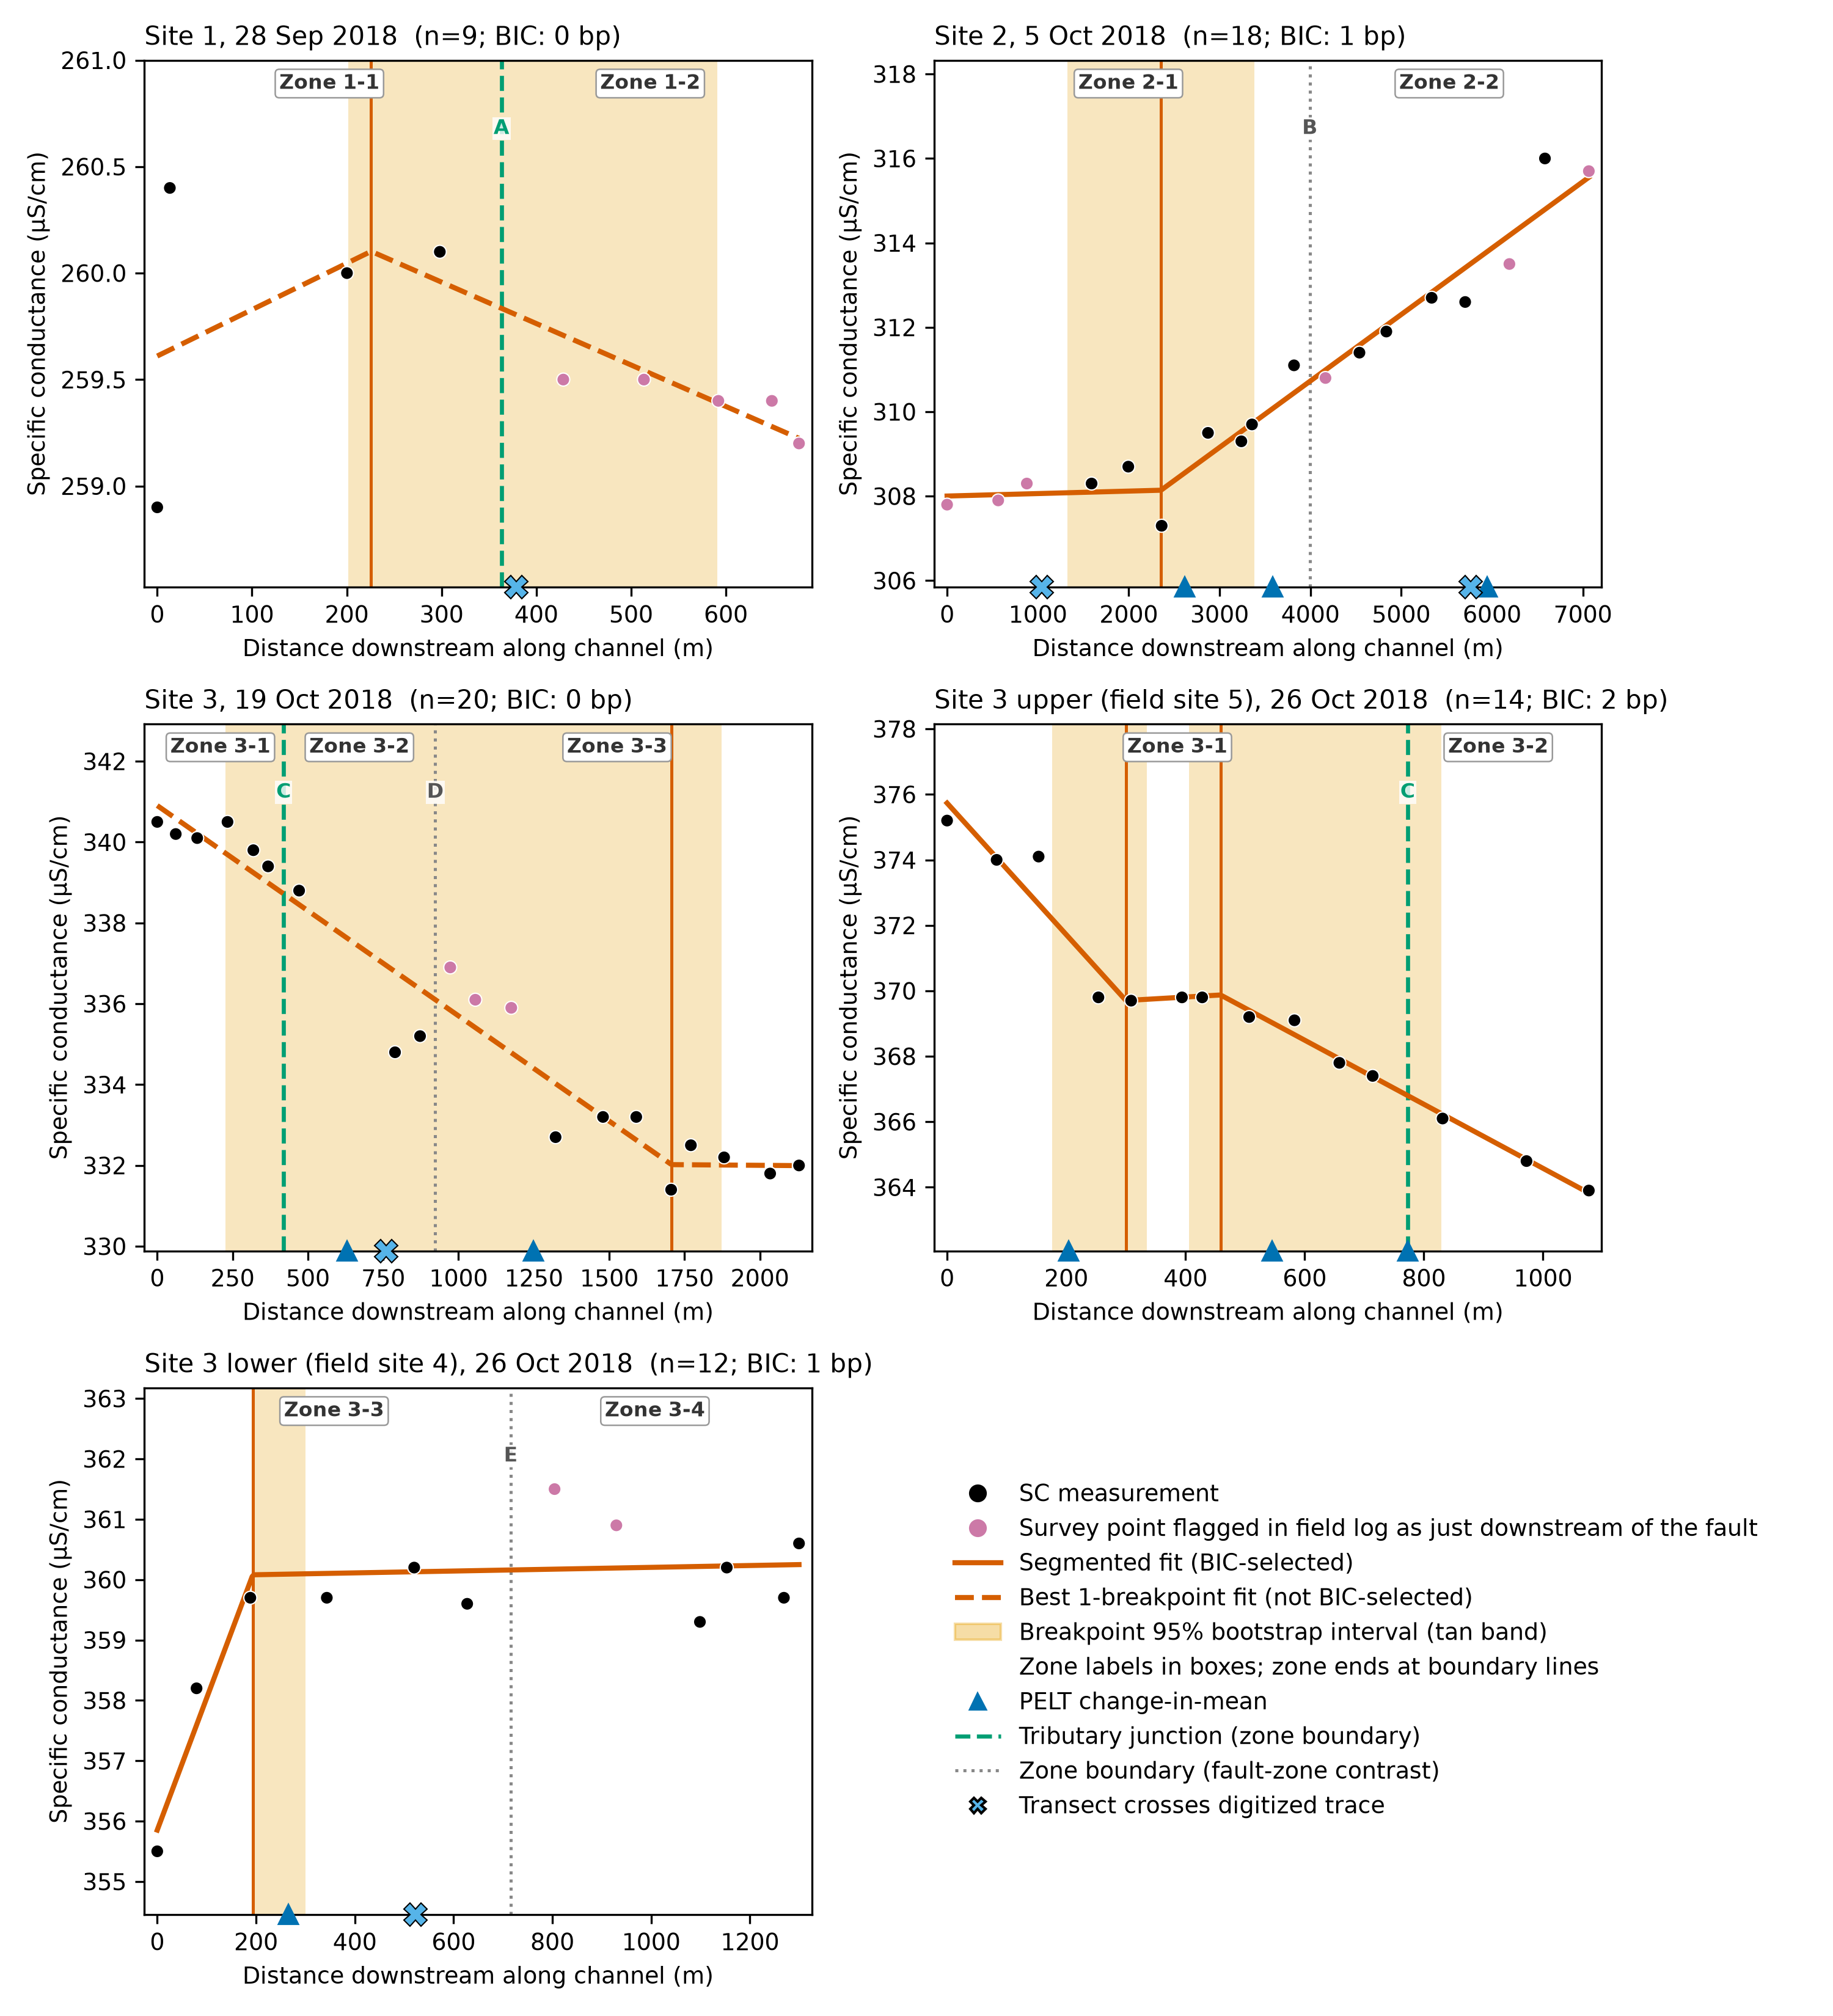
\includegraphics[width=\linewidth]{figures/rev_changepoint_sc.png}
	\caption{Specific conductance along each single-day transect, with segmented fits (orange) and 95\% breakpoint intervals (tan); where no breakpoint is selected, the best one-breakpoint fit is shown dashed, without an interval. Pink points are fault points; blue triangles are change-in-mean shifts; gray crosses are digitized fault-trace crossings; green and gray lines are tributary and fault-contrast zone boundaries.}
	\label{fig:changepoint}
\end{figure}

\subsection{Chloride transect}

\linelabel{L:cl-start}The 20 July 2020 transect (Figure~\ref{fig:chloride}) ran 2{,}351~m from Z to Z$'$, starting near the Contrast D fault points and ending just downstream of the Contrast E fault points, so it lies mostly within Zone 3-3. \linelabel{L:cl-peaks}Chloride across the 18 main-stem samples ranged from 13.75 to 50.0~mg/L, with the highest values at 474~m (50.0~mg/L), 690~m (36.25~mg/L) and 959~m (40.0~mg/L). These lie 133--468~m from the nearest Contrast D fault point and 293--391~m from the nearest digitized fault trace. The latter are straight-line distances; the transect itself crosses a digitized trace only once, at about 1.8~km (Figure~\ref{fig:chloride}). \linelabel{L:cl-bp}The segmented regression selects one breakpoint at 467~m (bootstrap interval 308--800~m), where the fitted slope changes from $+53$ to $-15$~mg/L per km; the change-in-mean analysis places shifts at 384 and 1021~m. Interestingly, the breakpoint is about 125~m from the nearest Contrast D fault point and about 300~m from the nearest trace; however, it is driven largely by the single 50~mg/L sample. \linelabel{L:cl-E}Near Contrast E, chloride is low and flat: only 2 of the 18 samples lie downstream of the Contrast E fault points (13.75 and 15.0~mg/L), and the last five samples are 13.75--17.5~mg/L. The transect therefore shows no chloride increase at Contrast E. With so few points downstream of E we did not attempt a two-sample test.

\begin{figure}[htbp]
	\centering
	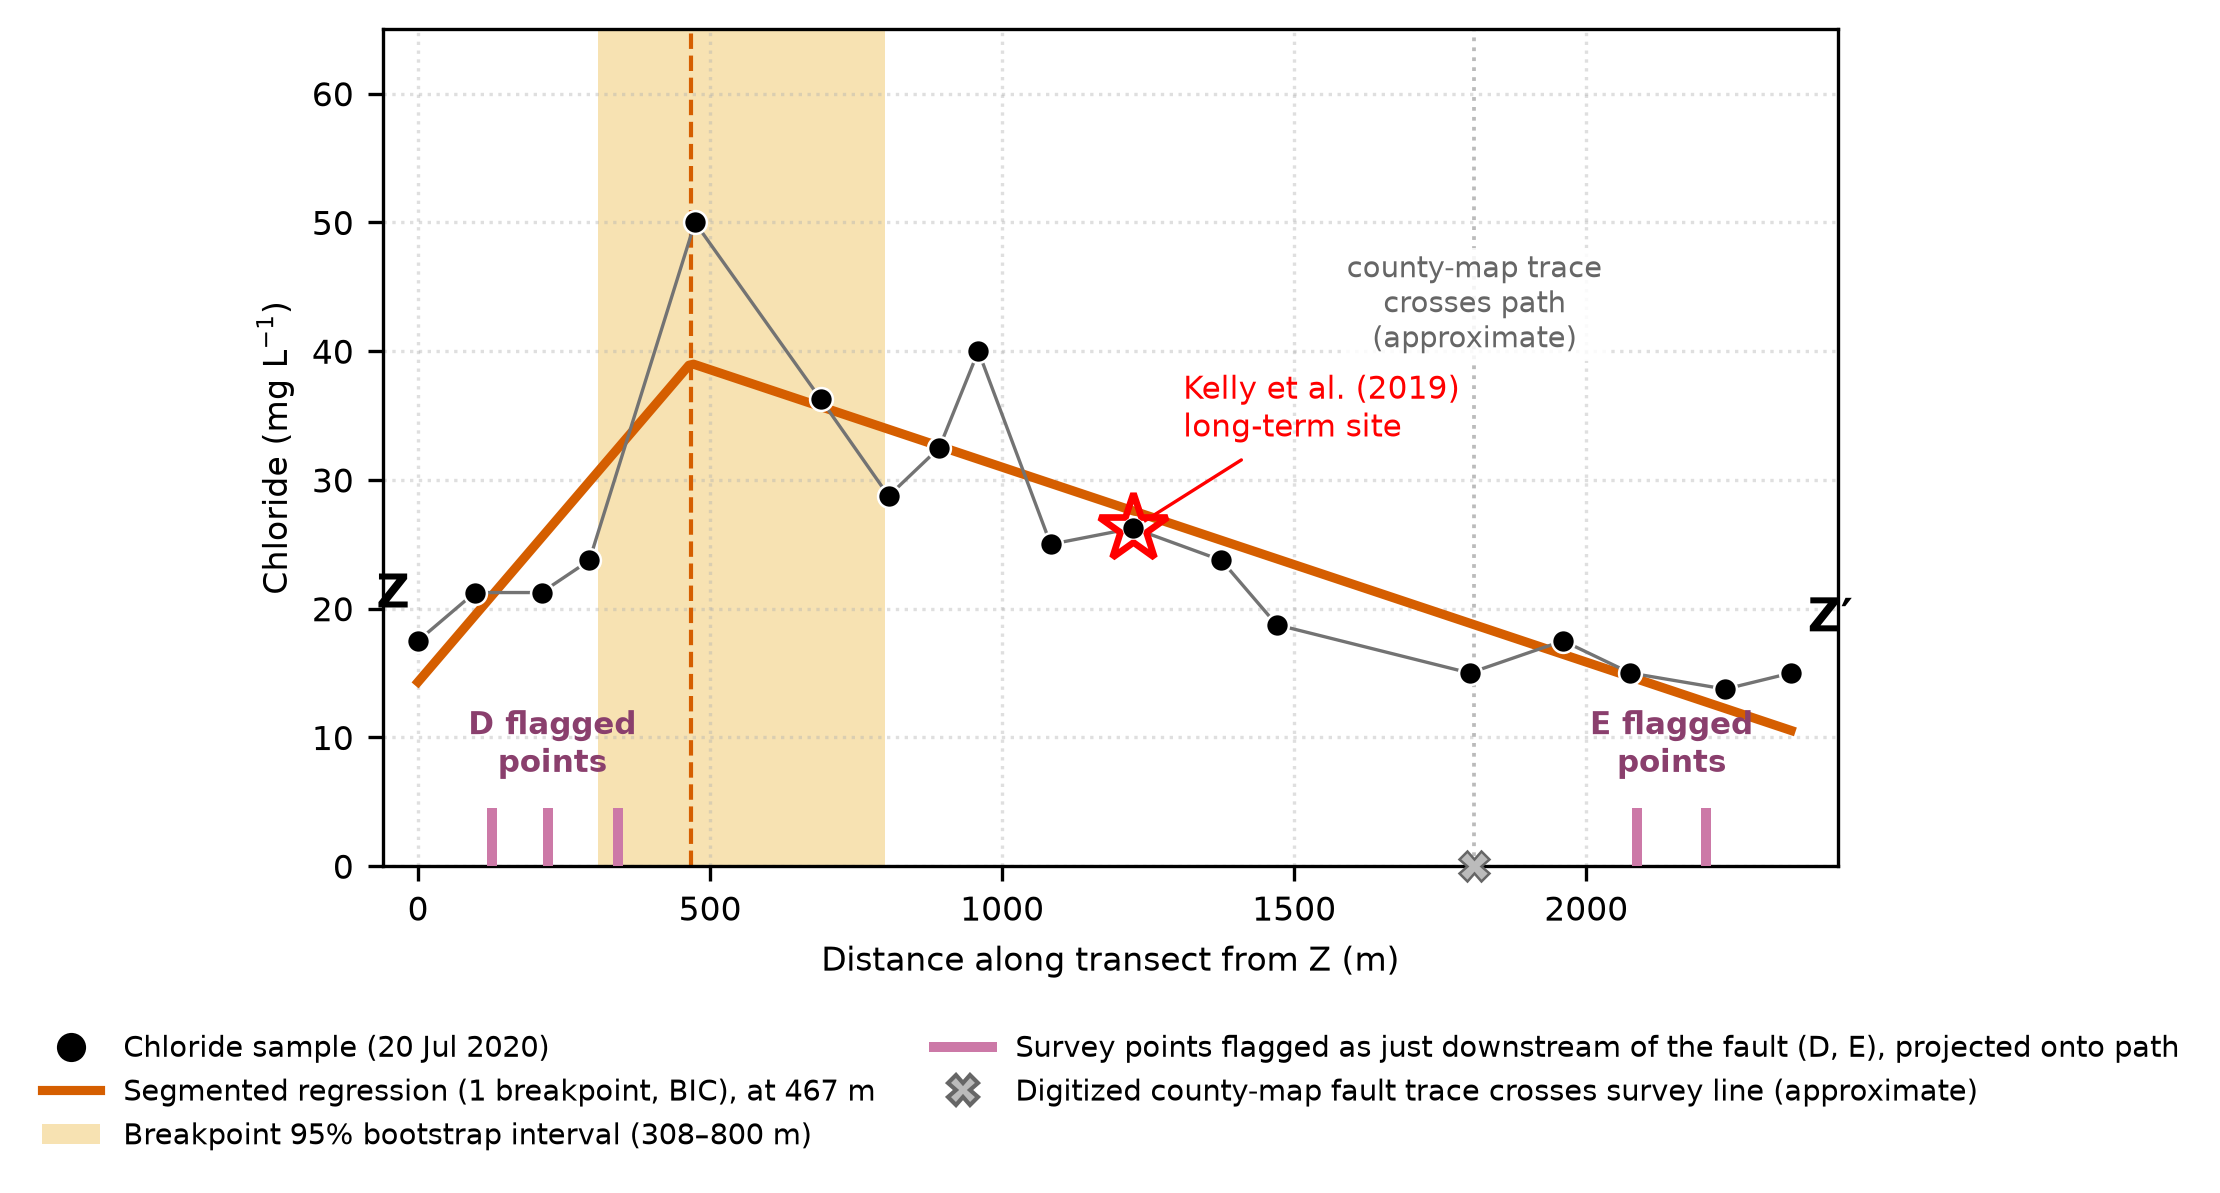
\includegraphics[width=0.9\linewidth]{figures/rev_chloride.png}
	\caption{Chloride along the 20 July 2020 transect (Z--Z$'$). The orange line is the segmented fit, with its breakpoint (467~m) and 95\% interval (tan); the breakpoint rests largely on the single 50~mg/L sample. Pink ticks mark the fault points at Contrasts D and E, the gray cross where the digitized fault trace crosses the transect, and the red star the monitoring site of \citet{kelly2019}.}
	\label{fig:chloride}
\end{figure}

\section{Discussion}

\subsection{What the contrasts show}\label{sec:disc-contrasts}

\linelabel{L:disc-answer}Our survey offers little support for the hypothesis that fault zones route road-salt-contaminated groundwater to Wappinger Creek. Of the three fault contrasts, one shows a small, significant increase in specific conductance (Contrast B, $+4.3$~$\mu$S/cm), one shows a non-significant decrease (Contrast D, $-2.8$~$\mu$S/cm) and one shows a non-significant increase within instrument accuracy (Contrast E, $+1.6$~$\mu$S/cm). No conductance breakpoint on any transect coincides with a fault contrast boundary. Recall that we set out three predictions in the Introduction. The first, an abrupt step at a fault, was not met at any crossing. \linelabel{L:disc-pred2}The second, persistence of the step at baseflow, could be examined only at Site 3, which was surveyed at baseflow on both days, and neither fault contrast there showed a significant increase; Sites 1 and 2 were surveyed at high flow, so Contrast B cannot speak to it. The third was examined only with a single chloride transect and no bromide. Hence, none of the three predictions is supported by this survey, although admittedly only the first could be examined at all three fault crossings.

Although Contrast B is statistically significant, we do not claim it as evidence of fault transport. The rise is gradual and begins roughly 1.6~km upstream of the zone boundary, which marks the fault position we interpreted in the field at an abrupt channel bend, along a reach where the county-scale fault trace runs parallel to the creek and cannot show where the fault meets the channel. A rise of this kind could be produced either by diffuse groundwater input or by a fault-parallel flowpath delivering water along the reach, and our survey cannot tell the two apart. Nevertheless, we believe Contrast B is an observation worth testing further, because it is the one place where conductance rose along a fault-controlled reach. \linelabel{L:disc-D}Contrast D, at a fault with no tributary, shows no increase. Indeed, on 19 October conductance fell steadily downstream through this boundary. \linelabel{L:disc-E}Contrast E is within the instrument's stated accuracy and its only breakpoint lies near the start of a short transect, 330~m upstream of where the channel crosses the trace. The 2020 chloride transect adds a further observation worth testing, in the same limited way: its peak lies near the Contrast D fault points and about 300~m from the nearest trace, but it rests on one sample, comes from a different year, and chloride near Contrast E is low (about 14--15~mg/L). \linelabel{L:disc-clpeak}We do not treat the chloride peak as support for the conductance result at any contrast.

The tributary contrast serves as an internal check, although admittedly a weak one. Conductance was lower below the junction on both days, which is the direction two-end-member mixing predicts when lower-conductance water joins the main stem \citep{genereux1998}. However, the downstream zone has only three points, the two tests disagree on 19 October, and conductance was already falling along the reach above the junction (Figure~\ref{fig:changepoint}), so we cannot say how much of the decrease the tributary itself supplies. Hence, we take Contrast C as an indication that the survey responds to a known input, and not as a measure of how small an input it can detect.

Furthermore, the differences we are discussing are small relative to what the instrument can resolve. The stated accuracy of the conductivity measurement is a bound on absolute error, and a calibration offset common to all readings on one day cancels in a within-day difference, but random reading error does not, and the manufacturer gives no repeatability figure. \linelabel{L:disc-size}Contrast B exceeds that bound by a factor of about 2.5 and exceeds the within-zone scatter, which is why we report it as a statistically significant but small difference; Contrast E does not exceed it. Site 1 contributes little either way, because a coincident tributary and very high flow after rain confound its only contrast. \linelabel{L:disc-screening}Taken together, the survey is best read as a screening result: it shows what a low-cost survey can detect, namely a small gradual rise at one site and the dilution at a tributary, and it also shows that such a survey does not locate a fault-related input to within the spacing of a few hundred meters that a fault trace of uncertain position would require.

\subsection{Alternative explanations}

\linelabel{L:alt-start}Several explanations for the Site 2 increase, and for the conductance differences generally, are at least as plausible as fault-routed groundwater with the data in hand.

We first considered the roads themselves. Per-zone median distances from survey points to the nearest major road range from 245 to 927~m (Table~\ref{tab:support}). \linelabel{L:alt-road-site2}At Site 2 the downstream zone is farther from a major road than the upstream zone (median 726 versus 335~m), so proximity to a major road does not by itself explain Contrast B, although one upstream point lies only 39~m from a road and the distances do not capture drainage or road density. The Site 3 zones lie 245--425~m from the nearest major road, mainly US 44, with no monotone relation to the conductance pattern. \linelabel{L:alt-road}These are descriptive medians, not a test, and they say nothing about salt stored in roadside soils and shallow groundwater, which may be flushed to the channel late in the season and which our survey cannot distinguish from deeper, fault-routed water. \linelabel{L:alt-season}Our surveys were made in late September and October, so a late-season release of such stored salt is a possibility we cannot exclude; it would, like diffuse groundwater, favor a gradual rise over a step.

Developed land is a second possible source, as stream conductance also rises near developed land from sources unrelated to faults or highways, such as residential runoff and lawn and agricultural fertilizers. Site 2 runs beside US 44 and ends near the settled area around Titusville (Figure~\ref{fig:site2}); we did not quantify land cover, and thus cannot weigh this source. Part of Site 3 lies within conserved forest (Section~\ref{sec:site}). \linelabel{L:alt-withdraw}Sampling within conserved land does not let us discount such inputs, because the sources lie in the contributing area and not only along the survey line.

Wastewater is a third possibility, and for Contrast B we believe it is the most specific one. \citet{kelly2008} estimated sodium chloride sources for the East Branch of Wappinger Creek and found that road salt contributed 83\% and parking-area salt 8\% (91\% from deicing), sewage including septic systems 4\%, and water softeners 3\%. We did not map septic systems along our reaches. The Millbrook sewage treatment plant that they describe is upstream of all three of our sites, about 2.4~km along the channel above Site 3 and 15.3 and 25.3~km above Sites 1 and 2 (facility locations from the US Environmental Protection Agency's Enforcement and Compliance History Online database, ECHO). As a continuous upstream source it would raise baseline conductance but would not by itself create a step at a zone boundary. More relevant to Contrast B, \linelabel{L:alt-wwtp}two small private plants, Stratford Farms and Ennis Mobile Home Park, have listed locations 240--370~m from Zone 2-1 (Figure~\ref{fig:site2}), at about 1.6 and 0.9~km along the survey, upstream of the 2{,}355~m breakpoint and, for the former, within its 1.3--3.4~km bootstrap interval. These are facility locations rather than outfalls, and flows are not listed, so we cannot test whether they contribute, but they are a plausible, untested alternative source for the Site 2 increase. The Titusville plant lies just downstream of the last Site 2 survey point, so it cannot affect Contrast B, and the Valley Dale plant discharges to a tributary about 2~km away, off the frame of Figure~\ref{fig:site2}. \linelabel{L:alt-troopk}A sixth listed facility, at a state police headquarters, lies about 0.8~km west of the downstream end of the Site 3 survey, on a tributary of the East Branch and not on the surveyed channel (the unlabeled square beside Site 3 in Figure~\ref{fig:overview}); no flow is listed for it.

Finally, groundwater unrelated to faults can enter the creek anywhere along a reach. Such diffuse inputs would raise conductance gradually downstream rather than in a step, and longitudinal surveys elsewhere show that local groundwater inputs and land use drive spatial variation in stream chloride \citep{hodgins2026}; the gradual ramp at Site 2 is consistent with such inputs. Long-term records show that stream chloride in the East Branch has risen from roughly 15~mg/L in the mid-1980s to over 40~mg/L by the mid-2000s \citep{kelly2008}, consistent with a regional anthropogenic source and a large store of salt in the subsurface \citep{vanmeter2024}, but a single monitoring location cannot show where along the channel that salt enters.

\subsection{Comparison with other studies and implications}

Our mixed result is not at odds with what is known about faults in rock like ours. The conduit--barrier model does not predict that every fault leaks, as a fault may carry water along its damage zone, block flow across its core, or do both, depending on its architecture and setting \citep{caine1996,bense2013}. In New England metamorphic bedrock, structural control has been shown at the scale of wells, through foliation-parallel fractures that raise connectivity and add anisotropy \citep{manda2008} and through a thrust fault that influences well yield and water chemistry \citep{kim2014}. Thus, a survey in which one of three faults shows a small rise and two show none does not tell us whether the other two faults act as barriers, are not connected to a source of salt, or simply discharge too little to register in the thalweg. These studies make fault-routed delivery plausible, but none of them involves road salt, and hence none of them tests it.

\linelabel{L:disc-surveys}Other longitudinal surveys locate salt-laden groundwater inputs more directly than ours. Electromagnetic mapping of a New Hampshire streambed found discrete reaches of high-conductivity discharge \citep{harte2010}, and streambed conductivity and temperature mapping in urban streams found porewater chloride ranging from under 100 to over 5{,}000~mg/L within about 10~m \citep{hodgins2024}. Longitudinal chloride and radon-222 in mixed-land-use streams showed that local groundwater inputs and land use drive spatial variation \citep{hodgins2026}, and long-term sampling of chloride in streams and springs has been used to trace groundwater-sourced road salt, with the highest chloride in a karst watershed in Pennsylvania occurring in summer baseflow \citep{orr2026}. Compared with these approaches, a thalweg survey at roughly 100--400~m spacing integrates over the whole channel flow and is presumably less sensitive to focused inputs that vary over 10~m. In other words, a survey like ours could miss a real fault signal as well as report a spurious one.

\linelabel{L:mgmt}We do not claim that the evidence here justifies changing deicing practice on the basis of fault locations. Mapped faults are, at most, a candidate screening layer, and future work should test them with the design in Section~\ref{sec:limits} before they are put to any use in salt management. Measures that reduce the total salt load, such as lower application rates, calibrated equipment, brine-based anti-icing and staff training, as recommended by the Adirondack Road Salt Reduction Task Force \citep{adirondack2023}, remain the better-supported response everywhere.


\subsection{Limitations and a test of the hypothesis}\label{sec:limits}

Admittedly, several limitations constrain how far these results can be taken. \linelabel{L:lim-discharge}We have no discharge measurements, so we cannot estimate the volume of any groundwater input, convert conductance to load, or separate dilution from addition. \linelabel{L:lim-tracers}We have no source tracers, so we cannot attribute salt to roads, wastewater or other sources. Future work with paired discharge and tracer measurements could address both of these gaps, as we describe at the end of this section.

\linelabel{L:lim-thalweg}Each reading is a single thalweg value, with no repeats across the channel or at depth, so lateral and vertical variation, which could exceed the small contrasts, is unmeasured. This matters because Contrasts B and E are close to the instrument's stated accuracy (Section~\ref{sec:disc-contrasts}), and we cannot rule out that reading error accounts for part of Contrast B. At Site 3 we surveyed on two days; the reach repeated on both days gave an offset that varied by about 6~$\mu$S/cm (Section~\ref{sec:contrasts}), too much to tie the days together, which limited us to within-day comparisons of small zones and left Contrast D untestable on 26 October.

The chloride data are more limited still, as they come from a single transect in a different year, measured with an ion-selective electrode whose stated accuracy ($\pm$15\% of reading or $\pm$5~mg/L) is a substantial fraction of the concentrations we measured; only the larger differences, such as the 50 and 40~mg/L peaks against a background of about 14--25~mg/L, exceed it. We therefore treat the chloride results as descriptive.

\linelabel{L:lim-faultpos}The fault traces come from a county-scale map for which no positional accuracy is stated (Section~\ref{sec:site}), so we cannot say how far a real fault lies from any mapped position. This is admittedly a weakness for a study whose hypothesis is spatial: if a mapped trace is off by a few hundred meters, a real step could fall outside the zone boundaries we tested. Field mapping of the fault zone at each crossing would remove this uncertainty. Moreover, our zones contain only three to eleven points, so the tests have little power and the autocorrelation used to discount them is itself poorly determined. Finally, three fault contrasts in one lithology cannot support a general statement about faults, and we leave it to future work with many crossings in several rock types to test whether any pattern holds.

\linelabel{L:td}The survey nonetheless suggests how the fault-conduit hypothesis could be tested. \linelabel{L:td-pitfall}Our Site 3 data show why surveys should be completed within a single day, or tied across days by repeated points at a steady offset: pooling the two survey days produces an apparent 18~$\mu$S/cm step at the second fault that is entirely the offset between days. Future work should pair each survey with discharge measurements, which would turn conductance into load and separate dilution from addition. Furthermore, chloride-to-bromide ratios would fingerprint deicing salt against wastewater and other sources \citep{mullaney2009}, while environmental age tracers would indicate whether water entering near a fault is older groundwater \citep{cook2022}. Repeated readings across the channel and at depth would show whether contrasts as small as ours exceed lateral variation. We also believe that fault zones should be located in the field rather than from county maps, and that change-point analysis should be applied to single-day transects so that gradual ramps and abrupt steps can be distinguished. Finally, surveys covering many crossings in several lithologies would show whether any pattern holds beyond one creek. We hypothesize that, if faults do route road salt to streams, such a design would find a step at a field-located fault that persists at baseflow and carries a deicing-salt signature and an older age; if it found none, the hypothesis could be set aside for faults of this kind.

\section{Conclusions}

In this work, we used longitudinal surveys of specific conductance and a single chloride transect to ask whether high-angle fault zones route road-salt-contaminated groundwater to Wappinger Creek, and our survey does not answer the question clearly. Comparing specific conductance within single survey days, we found a small but significant increase of 4.3~$\mu$S/cm at one of three fault contrasts (Site 2), about 2.5 times the instrument's stated accuracy. However, change-point analysis suggests that this increase is part of a gradual rise beginning roughly 1.6~km upstream of the channel bend where we placed the fault, rather than a step at it, and two private wastewater plants beside that reach offer an alternative explanation we could not test. At the other two faults, conductance either did not increase or rose by less than the instrument's accuracy, and no conductance breakpoint on any transect coincided with a fault contrast boundary. Conductance fell at the tributary junction, in the direction mixing predicts, which gives us some confidence that the survey responds to a known input. The single chloride transect from 2020 peaked near a different fault, but that peak rests on one sample.

We believe the most transferable result is methodological. When we pooled the two Site 3 survey days, the second fault appeared as the largest and most significant step in the survey (18.0~$\mu$S/cm), but within a single day the contrast was only $+1.6$~$\mu$S/cm; the apparent step was an artifact of the offset between days. Longitudinal surveys aimed at locating point inputs therefore need single-day sampling, or repeated points that tie survey days together at a steady offset, effective sample sizes that account for spatial autocorrelation, and analyses that can distinguish gradual ramps from abrupt steps.

Nevertheless, we do not think the hypothesis should be set aside. Studies of fault zones in fractured and metamorphic rock make fault-routed delivery plausible, and our survey could not have ruled it out, so we regard the hypothesis as plausible but unresolved. Until it is tested, we suggest that mapped faults be treated as a candidate screening layer to evaluate, and not as a basis for changing deicing practice. Future work should follow the design in Section~\ref{sec:limits}, with single-day surveys, discharge measurements and tracers, and should extend to other creeks and rock types to see whether any pattern holds.


\section*{Acknowledgements}

We would like to thank Marist University for providing funding and equipment to carry out our research as part of the first author's senior honors thesis and John Kittredge for collecting the data for the chloride samples within Figure~\ref{fig:chloride}. We also would like to thank the Cary Institute of Ecosystem Studies for allowing us access to walk sections of the East Branch of Wappinger Creek which fall under their property line.

\section*{Conflict of interest}

The authors declare that they have no conflict of interest.

\section*{Data Availability}

The data and code needed to reproduce the figures and statistics in this paper are available at the following GitHub Repository: \url{https://github.com/taddyb/wappingers_road_salts}. All individual specific-conductance measurements are also listed in Appendix~A. Road and stream layers are from the US Census Bureau TIGER/Line 2024 files and the USGS National Hydrography Dataset, and wastewater facility locations are from the EPA ECHO database (retrieved 2026-11-08).

\bibliographystyle{unsrtnat}
\bibliography{references_revised}


\appendix
\renewcommand{\thetable}{A\arabic{table}}
\setcounter{table}{0}
\renewcommand{\theHtable}{A\arabic{table}}

\section{Survey measurements}

Table~\ref{tab:appendix_data} \linelabel{L:appendix}lists every specific-conductance measurement from the 2018 survey: the survey and point number (Field and Pt; at Site 3, surveys 3, 5 and 4 are the 19 October, upper 26 October and lower 26 October surveys), the survey date, the along-channel distance from the upstream end of each single-day transect, the position, specific conductance (SC, $\mu$S/cm), water temperature ($T$, $^{\circ}$C), the zone, and whether the point is a fault point, located downstream of a fault (Fault: yes).

% Auto-generated by src/within_day.py. Requires \usepackage{longtable,booktabs}.
{\footnotesize
\begin{longtable}{rrrlrrrrrll}
\caption{All specific-conductance (SC) measurements, October 2018 survey. Distance is along-channel from the upstream end of each single-day transect (haversine sum of GPS fixes).}\label{tab:appendix_data}\\
\toprule Site & Field & Pt & Date & Dist (m) & Lat & Lon & SC & $T$ & Zone & Fault \\ \midrule \endfirsthead
\toprule Site & Field & Pt & Date & Dist (m) & Lat & Lon & SC & $T$ & Zone & Fault \\ \midrule \endhead
\bottomrule \endfoot
1 & 1 & 1 & 2018-09-28 & 0 & 41.80363 & -73.78189 & 258.9 & 15.3 & 1-1 & no \\
1 & 1 & 2 & 2018-09-28 & 13 & 41.80370 & -73.78202 & 260.4 & 15.2 & 1-1 & no \\
1 & 1 & 3 & 2018-09-28 & 200 & 41.80275 & -73.78388 & 260.0 & 15.2 & 1-1 & no \\
1 & 1 & 4 & 2018-09-28 & 298 & 41.80314 & -73.78494 & 260.1 & 15.2 & 1-1 & no \\
1 & 1 & 5 & 2018-09-28 & 428 & 41.80420 & -73.78561 & 259.5 & 15.2 & 1-2 & yes \\
1 & 1 & 6 & 2018-09-28 & 514 & 41.80359 & -73.78623 & 259.5 & 15.2 & 1-2 & yes \\
1 & 1 & 7 & 2018-09-28 & 592 & 41.80295 & -73.78663 & 259.4 & 15.2 & 1-2 & yes \\
1 & 1 & 8 & 2018-09-28 & 649 & 41.80251 & -73.78697 & 259.4 & 15.2 & 1-2 & yes \\
1 & 1 & 9 & 2018-09-28 & 677 & 41.80237 & -73.78726 & 259.2 & 15.2 & 1-2 & yes \\
2 & 2 & 1 & 2018-10-05 & 0 & 41.74113 & -73.83050 & 307.8 & 15.4 & 2-1 & yes \\
2 & 2 & 2 & 2018-10-05 & 563 & 41.73644 & -73.83305 & 307.9 & 15.4 & 2-1 & yes \\
2 & 2 & 3 & 2018-10-05 & 878 & 41.73422 & -73.83541 & 308.3 & 15.4 & 2-1 & yes \\
2 & 2 & 4 & 2018-10-05 & 1591 & 41.72798 & -73.83739 & 308.3 & 15.5 & 2-1 & no \\
2 & 2 & 5 & 2018-10-05 & 1995 & 41.72470 & -73.83949 & 308.7 & 15.6 & 2-1 & no \\
2 & 2 & 6 & 2018-10-05 & 2362 & 41.72140 & -73.83969 & 307.3 & 15.5 & 2-1 & no \\
2 & 2 & 7 & 2018-10-05 & 2872 & 41.71792 & -73.84369 & 309.5 & 15.6 & 2-1 & no \\
2 & 2 & 8 & 2018-10-05 & 3240 & 41.71499 & -73.84574 & 309.3 & 15.6 & 2-1 & no \\
2 & 2 & 9 & 2018-10-05 & 3357 & 41.71397 & -73.84609 & 309.7 & 15.6 & 2-1 & no \\
2 & 2 & 10 & 2018-10-05 & 3820 & 41.71455 & -73.85161 & 311.1 & 15.7 & 2-1 & no \\
2 & 2 & 11 & 2018-10-05 & 4166 & 41.71193 & -73.85387 & 310.8 & 15.7 & 2-2 & yes \\
2 & 2 & 12 & 2018-10-05 & 4540 & 41.70899 & -73.85606 & 311.4 & 15.7 & 2-2 & no \\
2 & 2 & 13 & 2018-10-05 & 4836 & 41.70650 & -73.85732 & 311.9 & 15.8 & 2-2 & no \\
2 & 2 & 14 & 2018-10-05 & 5335 & 41.70284 & -73.86080 & 312.7 & 15.8 & 2-2 & no \\
2 & 2 & 15 & 2018-10-05 & 5704 & 41.69994 & -73.86296 & 312.6 & 15.8 & 2-2 & no \\
2 & 2 & 16 & 2018-10-05 & 6191 & 41.69676 & -73.86699 & 313.5 & 15.7 & 2-2 & yes \\
2 & 2 & 17 & 2018-10-05 & 6582 & 41.69324 & -73.86698 & 316.0 & 15.8 & 2-2 & no \\
2 & 2 & 18 & 2018-10-05 & 7066 & 41.68951 & -73.86997 & 315.7 & 15.8 & 2-2 & yes \\
3 & 3 & 1 & 2018-10-19 & 0 & 41.79652 & -73.71534 & 340.5 & 9.4 & 3-1 & no \\
3 & 3 & 2 & 2018-10-19 & 61 & 41.79607 & -73.71577 & 340.2 & 9.4 & 3-1 & no \\
3 & 3 & 3 & 2018-10-19 & 133 & 41.79582 & -73.71656 & 340.1 & 9.5 & 3-1 & no \\
3 & 3 & 4 & 2018-10-19 & 233 & 41.79613 & -73.71770 & 340.5 & 9.5 & 3-1 & no \\
3 & 3 & 5 & 2018-10-19 & 319 & 41.79673 & -73.71835 & 339.8 & 9.6 & 3-1 & no \\
3 & 3 & 6 & 2018-10-19 & 368 & 41.79674 & -73.71894 & 339.4 & 9.5 & 3-1 & no \\
3 & 3 & 7 & 2018-10-19 & 471 & 41.79639 & -73.72009 & 338.8 & 9.6 & 3-2 & no \\
3 & 3 & 8 & 2018-10-19 & 789 & 41.79467 & -73.72316 & 334.8 & 9.7 & 3-2 & no \\
3 & 3 & 9 & 2018-10-19 & 872 & 41.79394 & -73.72337 & 335.2 & 9.7 & 3-2 & no \\
3 & 3 & 10 & 2018-10-19 & 973 & 41.79374 & -73.72455 & 336.9 & 9.7 & 3-3 & yes \\
3 & 3 & 11 & 2018-10-19 & 1056 & 41.79331 & -73.72537 & 336.1 & 9.7 & 3-3 & yes \\
3 & 3 & 12 & 2018-10-19 & 1175 & 41.79251 & -73.72633 & 335.9 & 9.8 & 3-3 & yes \\
3 & 3 & 13 & 2018-10-19 & 1322 & 41.79155 & -73.72755 & 332.7 & 10.0 & 3-3 & no \\
3 & 3 & 14 & 2018-10-19 & 1479 & 41.79168 & -73.72944 & 333.2 & 10.0 & 3-3 & no \\
3 & 3 & 15 & 2018-10-19 & 1590 & 41.79136 & -73.73070 & 333.2 & 10.0 & 3-3 & no \\
3 & 3 & 16 & 2018-10-19 & 1706 & 41.79091 & -73.73196 & 331.4 & 10.0 & 3-3 & no \\
3 & 3 & 17 & 2018-10-19 & 1771 & 41.79048 & -73.73142 & 332.5 & 10.1 & 3-3 & no \\
3 & 3 & 18 & 2018-10-19 & 1881 & 41.78949 & -73.73137 & 332.2 & 10.1 & 3-3 & no \\
3 & 3 & 19 & 2018-10-19 & 2034 & 41.78819 & -73.73197 & 331.8 & 10.2 & 3-3 & no \\
3 & 3 & 20 & 2018-10-19 & 2130 & 41.78765 & -73.73287 & 332.0 & 10.2 & 3-3 & no \\
3 & 5 & 14 & 2018-10-26 & 0 & 41.79600 & -73.71273 & 375.2 & 8.7 & 3-1 & no \\
3 & 5 & 13 & 2018-10-26 & 83 & 41.79581 & -73.71370 & 374.0 & 8.7 & 3-1 & no \\
3 & 5 & 12 & 2018-10-26 & 154 & 41.79640 & -73.71401 & 374.1 & 8.7 & 3-1 & no \\
3 & 5 & 11 & 2018-10-26 & 254 & 41.79660 & -73.71519 & 369.8 & 8.8 & 3-1 & no \\
3 & 5 & 10 & 2018-10-26 & 309 & 41.79614 & -73.71543 & 369.7 & 8.8 & 3-1 & no \\
3 & 5 & 9 & 2018-10-26 & 394 & 41.79573 & -73.71630 & 369.8 & 8.7 & 3-1 & no \\
3 & 5 & 8 & 2018-10-26 & 428 & 41.79556 & -73.71664 & 369.8 & 8.7 & 3-1 & no \\
3 & 5 & 7 & 2018-10-26 & 507 & 41.79607 & -73.71730 & 369.2 & 8.8 & 3-1 & no \\
3 & 5 & 6 & 2018-10-26 & 583 & 41.79652 & -73.71799 & 369.1 & 8.8 & 3-1 & no \\
3 & 5 & 5 & 2018-10-26 & 658 & 41.79688 & -73.71876 & 367.8 & 8.8 & 3-1 & no \\
3 & 5 & 4 & 2018-10-26 & 714 & 41.79656 & -73.71928 & 367.4 & 8.8 & 3-1 & no \\
3 & 5 & 3 & 2018-10-26 & 831 & 41.79620 & -73.72061 & 366.1 & 8.7 & 3-2 & no \\
3 & 5 & 2 & 2018-10-26 & 972 & 41.79515 & -73.72156 & 364.8 & 8.8 & 3-2 & no \\
3 & 5 & 1 & 2018-10-26 & 1077 & 41.79478 & -73.72272 & 363.9 & 8.9 & 3-2 & no \\
3 & 4 & 1 & 2018-10-26 & 0 & 41.78772 & -73.73268 & 355.5 & 8.3 & 3-3 & no \\
3 & 4 & 2 & 2018-10-26 & 80 & 41.78704 & -73.73298 & 358.2 & 8.2 & 3-3 & no \\
3 & 4 & 3 & 2018-10-26 & 188 & 41.78674 & -73.73423 & 359.7 & 8.2 & 3-3 & no \\
3 & 4 & 4 & 2018-10-26 & 343 & 41.78550 & -73.73508 & 359.7 & 8.1 & 3-3 & no \\
3 & 4 & 5 & 2018-10-26 & 520 & 41.78416 & -73.73623 & 360.2 & 8.1 & 3-3 & no \\
3 & 4 & 6 & 2018-10-26 & 628 & 41.78364 & -73.73732 & 359.6 & 8.2 & 3-3 & no \\
3 & 4 & 7 & 2018-10-26 & 804 & 41.78239 & -73.73864 & 361.5 & 8.1 & 3-4 & yes \\
3 & 4 & 8 & 2018-10-26 & 930 & 41.78302 & -73.73989 & 360.9 & 8.1 & 3-4 & yes \\
3 & 4 & 9 & 2018-10-26 & 1099 & 41.78305 & -73.74193 & 359.3 & 8.3 & 3-4 & no \\
3 & 4 & 10 & 2018-10-26 & 1153 & 41.78323 & -73.74254 & 360.2 & 8.3 & 3-4 & no \\
3 & 4 & 11 & 2018-10-26 & 1269 & 41.78308 & -73.74392 & 359.7 & 8.4 & 3-4 & no \\
3 & 4 & 12 & 2018-10-26 & 1299 & 41.78325 & -73.74421 & 360.6 & 8.3 & 3-4 & no \\
\end{longtable}
}


\end{document}
